\documentclass[
	12pt,
	a4paper,
	ngerman,
	oneside,
]{article}

\usepackage[utf8]{inputenc}						%Umlaute etc
\usepackage[style=alphabetic, backend=biber]{biblatex} 	%bibtex
\usepackage[babel,german=quotes]{csquotes} 			%bibtex
\addbibresource{literaturverzeichnis.tex} 				%bibtex

\usepackage[ngerman]{babel} 						%Dokument Deutsch
\usepackage[onehalfspacing]{setspace} 				%Zeilenabstand
\usepackage{caption} 
\usepackage{tabularx}							%Tabellen
\usepackage{listings} 								%Code
\usepackage{graphicx} 							%Grafiken
\usepackage{picins}
\usepackage{wrapfig}
\usepackage{listings}
\usepackage[usenames]{color} 						%Farben
\usepackage[hidelinks]{hyperref} 					%Links in Dokument
\usepackage{fancyhdr}
\usepackage[official]{eurosym}
\lstset{  										%Codesettings
  basicstyle=\ttfamily\footnotesize,
  commentstyle=\color{red},
  keywordstyle=\color{blue},
  numbers=left,
  showstringspaces=false,
  breaklines=true,
  frame=single,
  tabsize=2
}
\lstdefinelanguage{conf} 							%Extrasettings
{
    morecomment=[l]{\#}
}

\pagestyle{fancy}
\fancyhf{}
\rhead{Seite \thepage}


\begin{document}


\begin{titlepage}

  \author{Silas Leidel, Dennis Hufnagel, Marcel Fuchs, Michael Kainz\\\\Betreut von Prof. Dr. Klehn}
  \title{Automatisierte Bewässerungsanlage für Indoor Pflanzen}
  \date{\today}
  \maketitle
\end{titlepage}

\newpage
\setcounter{page}{2}
\tableofcontents
\newpage

\section{Vorwort}
\subsection{Problemstellung}

Auf dem Markt existieren schon alle möglichen Bewässerungssysteme. Von Rasenbewässerungen bis zu Topfpflanzen ist alles vertreten. Die meisten Systeme existieren für die Gartenbewässerung (zum Beispiel von Gardena) und werden an
die Wasserleitung mit 1/2 Zoll direkt angeschlossen. Die Steuerungen sind eher einfach gehalten. Einstellbar sind die Wassermenge und die Bewässerungszeitpunkte. Bei den Lösungen für Beete und Kübel ist eine Steuerung eher selten. Sie erfolgt
durch das Auf- und Zudrehen der Wasserzufuhr. Aus dieser Marktlage folgernd, wird in diesem Projekt ein Bewässerungssystem für Topf- und Beetpflanzen geplant und realisiert.

\subsection{Projektziel}
Das System soll eine Regelung enthalten, die mindestens dieselben Funktionen enthalten soll, wie die bereits bestehenden Produkte. Zusätzlich soll durch  ein oder zwei Feuchtigkeitssensoren die Feuchtigkeit in die Steuerung einfließen
und somit zur Regelung wird. Die Wasserzufuhr soll wahlweise über ein separates Wasserreservoir oder über einen Standardwasseranschluss zur Verfügung gestellt werden. Die gemessenen Daten werden in einem Arduinoboard, welches die
zentrale Mikrocontrollereinheit ist, zusammengeführt und ausgewertet. Die Daten und Änderungen im Bewässerungszyklus können über eine Wlanschnittstelle entnommen und verändert werden. Die Schnittstelle wird über ein ESPboard realisiert.
Die Kosten der Materialen soll um 200 \euro{} liegen.

\section{Aufgabenteilung}
Das Projektteam besteht aus vier Mitarbeitern. Es sind dementsprechend vier Aufgabengebiete erstellt worden. Das erste Gebiet umfasst den Aufbau und die Implementierung der Sensoren. Hierfür verantwortlich ist Dennis Hufnagel.
Der nächste Bereich ist die Wasser- und Stromversorgung. Dort ist Silas Leidel verantwortlich. Den dritten Bereich, welcher die Realisation der Steuerung im Arduino umfasst, betreute Marcel Fuchs. Die WLAN-Schnittstelle und
die Konfiguration des ESPboards übernimmt Michael Kainz.

\begin{figure}[ht]
    \centering
    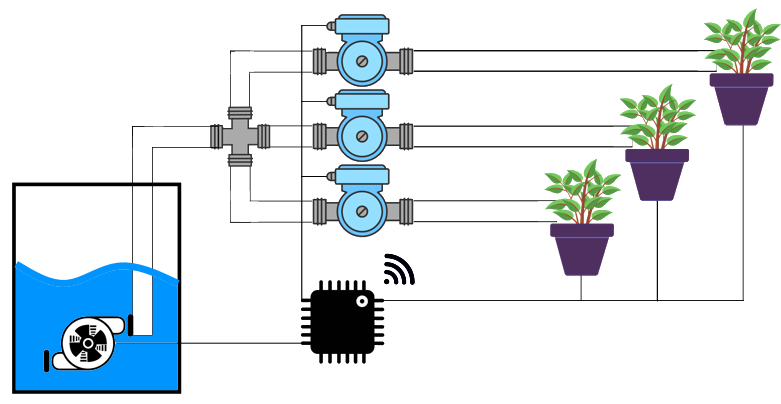
\includegraphics[width=\textwidth]{silas/blockschaltbild}
    \caption{Schema der Anlage}
\end{figure}
\newpage
\fancyhf{}
\lhead{Silas Leidel}
\rhead{Seite \thepage}

\section{Wasserversorgung}

\subsection{Planung/ Realisation}
Da das Projekt für Beete und Töpfe geplant ist, ist die benötigte Wassermenge pro einmaliger
Wässerung und über einige Zyklen überschaubar.Am Beispielfall der Orchidee, eine der beliebtesten
Zimmerpflanzen in Deutschland, wird
der Wasserverbrauch verdeutlicht. Eine Orchidee sollte im Sommer zweimal wöchentlich gegossen werden.
 Bei jedem Gießvorgang werden ca. 100ml Wasser verbraucht. Bei drei Pflanzen liegt der Wasserverbrauch
 bei 600ml in der Woche. Die meisten
anderen beliebten Zimmerpflanzen, wie z.B. der Gummibaum, benötigen weniger Wasser. Aus diesem
Beispiel sieht man, das ein externes Wasserreservoir vollkommen ausreichend ist. So kann ein
5l-Kanister auf Basis der Berechnung
das System für 8 Wochen mit Wasser versorgen. Wenn die benötigte Wassermenge höher ist oder der
Wiederbefüllungszyklus größer sein soll, kann ein größerer Kanister als Wasserspeicher genutzt
werden. Zudem besteht bei einer
Innenanlage das Problem der Anschlussrealisierungen an die Haustrinkwasserleitung. Aufgrund dieser
Überlegungen ist ein Kanister eingeplant.
Das Wasser aus dem Kanister muss zu den Pflanzen transportiert werden. Die einfachste Lösung ist
die Nutzung der potentiellen Energie um die Pflanzen zu versorgen. Das Reservoir wird auf ein höheres
Niveau gestellt als die
Verteilungsanlage. Alternativ kann das Wasser durch eine Pumpe aus dem Speicher verteilt werden.
Bei der Betrachtung der Realisierung mit dem Niveauunterschied ergaben sich diverse Probleme. Zum einen ist der Wasserdruck nicht
konstant. Der Druck ist abhängig von dem Niveauunterschied und von der enthaltenen Wassermenge im
Speicher. Da kein Mengenzähler vorgesehen ist, wird die abgegebene Wassermenge durch die
Freischaltung bestimmt und reguliert. Bei
unbestimmten Druck variiert die Wassermenge zu stark. Deshalb wird eine Pumpe für den Transport
präferiert. Eingesetzt wird eine kleine Pumpe aus dem Campingbedarf mit einer Fördermenge
von $600\frac{l}{h}$ und einem Druck von $0,5 bar$.
Diese Pumpe darf zwar nur eine halbe Stunde am Stück laufen, jedoch sind solch hohe Laufzeiten
sowieso nicht gefordert.
Die Wahl bei den Schläuchen fiel auf Polyurethanschläuche. Diese werden in der Pneumatik eingesetzt.
Mit der Wahl dieser Schläuche kann man gleichzeitig die Vorteile von Pneumatiksystemen nutzen.
Besonders hervorzuheben ist die
hohe Druckfestigkeit bis $7 bar$ und die Nutzung von Stecksystemen. Zur Verteilung auf die einzelnen
Pflanzen wird ein 4-Wege Pneumatikverteiler genutzt. Der Verteiler besitzt eine klassische
Steckverbindung. Die sorgt für den
dichten Anschluss der Schläuche. Der Außendurchmesser beträgt $10mm$ und der Innendurchmesser $8mm$.
Dieser Durchmesser wurde aufgrund des $10mm$ Anschlusses der Pumpe gewählt.
Zur Schaltung des Wassers werden Magnetventile verwendet. Für die 1/2 Zoll Gewinde des Magnetventiles
wird auf der Verteilerseite mit einem Steckverbindungsfitting gearbeitet. Schlauchtüllen mit $10mm$
Durchmesser werden auf der Pflanzenseite benutzt.

\begin{figure}[ht]
    \centering
    %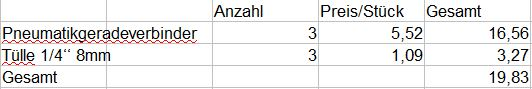
\includegraphics[width=\textwidth]{silas/preis}
    \begin{tabular}{|l|r|r||r|}
        \hline
        & Anzahl & Preis/Stück & Gesamt \\\hline
        Pneumatikgeradeverbinder & 3 & 5,52 & 16,56 \\\hline
        Tülle 1/4'' 8mm & 3 & 1,09 & 3,27 \\\hline
        Gesamt & & & 19,83 \\\hline
    \end{tabular}
    \caption{Preise von Schlauchzubehör}
\end{figure}


Die Entscheidung gegen die Steckverbindungsfittings
auf allen Seiten wurde wegen des Preises getroffen.
Der Preisvorteil liegt bei ca. 4 \euro{} und mit drei Teilen bei 12 \euro{} .
Die Schraubverbindungen sind alle nicht konisch ausgeführt. Dadurch sind die Verbindungen nicht selbstdichtend. Damit diese trotzdem verwendet werden können, wird Teflonband um die Gewinde gewickelt. Von den Tüllen werden die
Schläuche dann in die zu versorgenden Pflanzen gesteckt.

\subsection{Probleme bei der Realisation}
Bei der Montage und Realisierung sind einige Probleme aufgetreten. So hat der Schlauch nicht auf
die Fassung der Pumpe gepasst. Deshalb wurde ein Aquaristikschlauch mit einem
Außendurchmesser $12mm$ und einem Innendurchmesser von
$9mm$ genutzt. Die Fixierung erfolgte durch Schlauchklemmen, die an der Pumpe und am Übergang
zu dem Polyurethanschlauch für die sichere Verbindung sorgen. Ein weiteres Problem war das
Auffinden des passenden Kanisters. Herkömmliche
Kanister, wie zum Beispiel für destilliertes Wasser, haben eine Öffnung von $35mm$. Durch diese
Öffnung ist die Pumpe nicht versenkbar. Deshalb musste ein spezieller Kanister mit einer
Weithalsöffnung von $88mm$ besorgt werden.
Zusätzlich waren die Polyurethanschläuche nicht sehr flexibel, weshalb der Verteiler etwas
weiter entfernt platziert werden muss, um die erhöhten Biegeradien einzuhalten.

\section{Stromversorgung}

\subsection{Planung/Realisation}
Die erste grundsätzliche Frage, die zu klären war, ist, ob die Stromversorgung über ein Solarpanel
oder über ein Netzteil erfolgt. Deshalb wurden erstmal alle Verbraucher mit ihren elektrischen K
enndaten bestimmt. Zusätzlich wurde
die Betriebsdauer an einem Tag der Teile festgesetzt.


\begin{figure}[ht]
    \centering
    %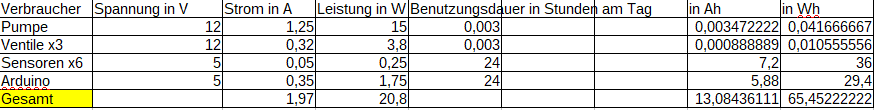
\includegraphics[width=\textwidth]{silas/verbrauch}
    \begin{tabular}{|l|r|r|r|r|r|r|}
        \hline
        Verbraucher & Spannung & Strom & Leistung & Dauer & in Ah & in Wh \\\hline\hline
        Pumpe & 12V & 1,25 & 15 & 0,003 & 0,003472 & 0,4166 \\\hline
        Ventile x3 & 12V & 0,32 & 3,8 & 0,003 & 0,00088 & 0,01055 \\\hline
        Sensoren x6 & 5 & 0,05 & 0,25 & 24 & 7,2 & 36 \\\hline
        Arduino & 5 & 0,35 & 1,75 & 24 & 5,88 & 29,4 \\\hline
        Gesamt &  & 1,97 & 20,8 &  & 13,0843 & 65,452 \\\hline
    \end{tabular}
    \caption{Stromverbrauch der Komponenten}
\end{figure}

Es gibt zwei Versorgungsspannungen.
Mit $12V$ wird das Arduinoboard versorgt. Um die benötigten Potentiale so gering wie
möglich zu halten, wurden die anderen Bauteile auch mit $12V$
Betriebsspannung ausgesucht. Nur für die Sensoren werden $5V$ benötigt.
Aus der Abbildung ist zu entnehmen, das die großen Verbraucher, wie die Pumpe und die Ventile,
nur die maximale Momentanleistung und damit den maximalen Momentanstrom festlegen. Für die
benötigte Gesamtleistung sind die dauerlaufenden Bauteile viel entscheidender.
Auf Basis der Leistungswerte und der Faustformel für
Solarpanels $W_{peak} * 4 = W_{tag}$ wird ein Panel mit mindestens $30W_{peak}$ benötigt. Das
hier eingeplante Panel \footnote{https://www.offgridtec.com/offgridtecr-30w-mono-$12V$-solarpanel.html}
bringt mehrere Probleme mit sich. So sind die
Abmessung von $340x605mm$ schwer in ein schlankes Gehäuse zu integrieren. Des weiteren sind die
Kosten wieder mitentscheidend. Für die Panellösung
muss zusätzlich ein Laderegler (ca.10-20 \euro{}) und eine Batterie(ca. 10-20 \euro{}) besorgt werden.
Im Vergleich zu dem dann letztendlich verwendeten Netzteil mit Kabel (21,25 \euro{}) liegt der
Preisnachteil bei ca. 45-55 \euro{}. Das Netzteilkabel liefert
durch eine Steckerbuchse den Strom an die Komponente. Die maximale Strommenge des Netzteil beträgt
$2,5 A$ und die maximale Leistung $30W$.
Da die Pumpen und Ventile mit dem Arduino geschalten werden, ist eine Schaltplatine notwendig.
Dazu kommt noch eine Platine, worauf die Spannungen zur Verfügung gestellt werden.

\subsection{Verteilerplatine}

\begin{figure}[ht]
    \centering
    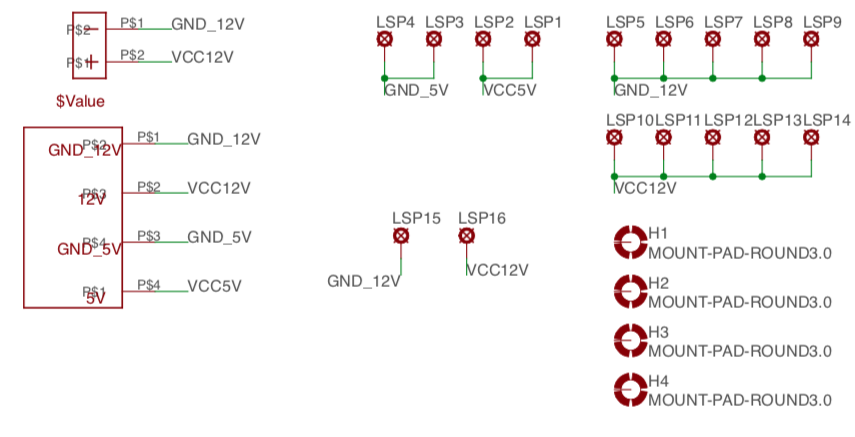
\includegraphics[width=\textwidth]{silas/verteiler1}
    \caption{Schaltplan der Verteilerplatine}
\end{figure}

In diesem Teil wird nur die Schaltungsplanung erläutert. Die Layouterstellung wird in einem späteren
Kapitel erklärt.
Die geplante Verteilerplatine soll die zwei Versorgungsspannungen zur Verfügung stellen.
Mittels eines DC-Jack werden die $12V$ von dem Netzteil auf die Platine geführt.
Von dort wird mittels eines DC/DC-Wandlers die Spannung auf $5V$
heruntergesetzt. Der Wandler hat vier Anschlussstifte. Zwei für $VCC$ $12V$ und $GND$ $12V$ und zwei
weitere für $VCC$ $5V$ und $GND$ $5V$. Von dem $5V$ Versorgungsbereich werden Abgänge zu der
Schaltplatine geplant. Ebenso gibt es Abgänge von dem $12V$ Niveau.
Die Masse des Netzteiles und der Platine sind durch den DC-Jack schon miteinander verbunden.
Zusätzlich wird die vom Wandler gestellte $5V$-Masse mit der Netzteilmasse verbunden. Dadurch
entsteht eine gemeinsame Masse und falsche Bezugspotentiale
werden ausgeschlossen. Auf jedem Potential wurde mindestens ein Reservelötloch eingeplant.
Das Arduinoboard wird über einen direkt eingelöteten DC Jackstecker versorgt.

\subsection{Schaltplatine}

\begin{figure}[ht]
    \centering
    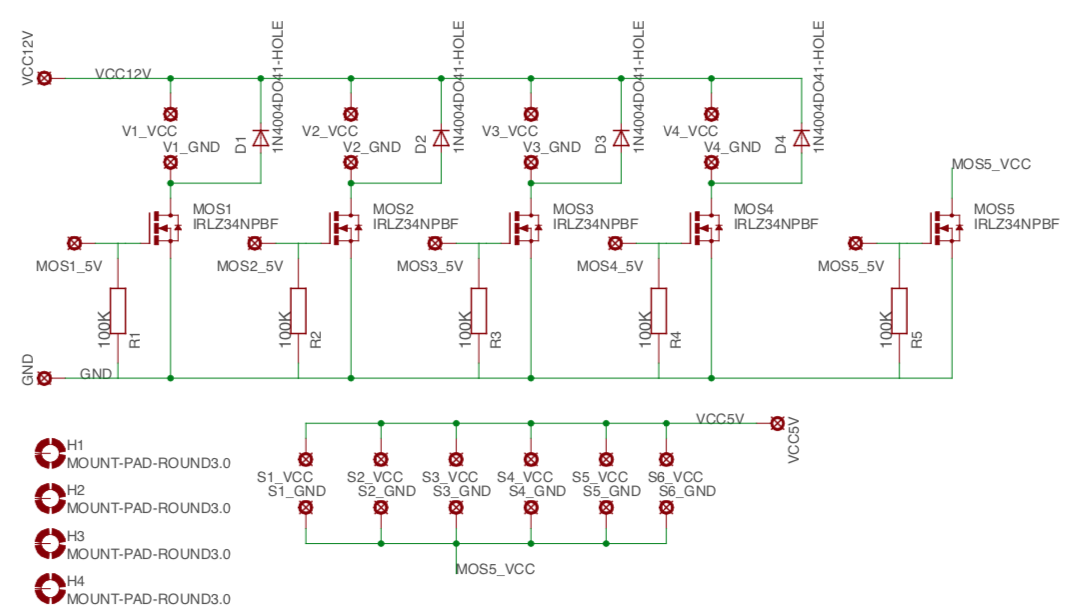
\includegraphics[width=\textwidth]{silas/versorgung1}
    \caption{Schaltplan der Versorgungsplatine}
\end{figure}

In diesem Teil wird nur die Schaltungsplanung erläutert. Die Layouterstellung wird in einem
späteren Kapitel erläutert.
Die Pumpen und die Ventile sollen durch einen Befehl des Arduinos einzeln an- und ausgeschalten
werden können. Die Sensoren sollen wegen Energiesparmaßnahmen gemeinsam ausgeschaltet werden können.
Als Schalter wird der Mosfet IRLZ34NPBF verwendet. Wichtig
ist, dass der Mosfet bei $5V$ Spannung durchschaltet und nicht höhere Threshholdspannungen benötigt.
Das Arduino kann nur $5V$ an den Pins liefern. Da induktive Lasten geschalten werden, muss eine
Freilaufdiode eingebaut werden. Darüber
baut sich Spannungsspitze der Selbstinduktion nach dem Ausschalten ab und schützt somit den Mosfet.
Parallel zu der Diode wird das induktive Bauteil eingesetzt. Die $100k\Omega$ Widerstände wirken
Pull-Down-artig. Damit wird garantiert das
der Mosfet immer sicher sperrt. Für die Sensoren wird keine Freilaufdiode benötigt,
weil hier nur geringe kapazitive Lasten zum tragen kommen.

\section{Gehäuse}
In dem Gehäuse soll die ganze Elektrik, Ventile un der Wasserverteiler verbaut werden.
Die Maße wurden durch die Biegeradien der Schläuche vorgegeben. Die somit ermittelten
Abmaße sind $350x300x100mm$. Als Material wurden herkömmliche Sieb-
druckplatten aus dem Baumarkt verwendet. Diese wurden zugeschnitten und mit Metallwinkeln
zu einem Kasten verbunden. Der Deckel wurde mit Scharnieren montiert. Die Ventile sind
auf Winkeln montiert und jederzeit entnehmbar. Der Verteiler
ist hingegen mit Schrauben direkt an der Bodenplatte befestigt. Für die Schläuche sind
Löcher mit $10mm$ Durchmesser in die Wand gebohrt worden. Diese Löcher wurden noch etwas
ausgefeilt, weil die Schläuche schwer durch zu bewegen waren.
Auf jeder Seite, wo schon Löcher vorhanden sind, wurden noch welche für die Leitungen gebohrt.
Auf der Zuführungsseite wurde das Leitungsloch größer mit $13mm$ Durchmesser, denn der Stecker
vom Netzteil wird durch diese Bohrung geführt.
Die Elektrik ist in einem Kunststoffkasten gekoffert. Der Kasten hat die Abmaße von $185x105x61mm$
und ist an den Deckel des Gehäuses festgeschraubt. Hier mussten auch auf zwei gegenüberliegenden
Seiten Löcher für die Leitungen gebohrt werden.
Auf der einen Seite ist die Stromzuführung und auf der anderen sind die Abgänge für die Ventile
beziehungsweise Sensoren.
\begin{figure}
    \centering
    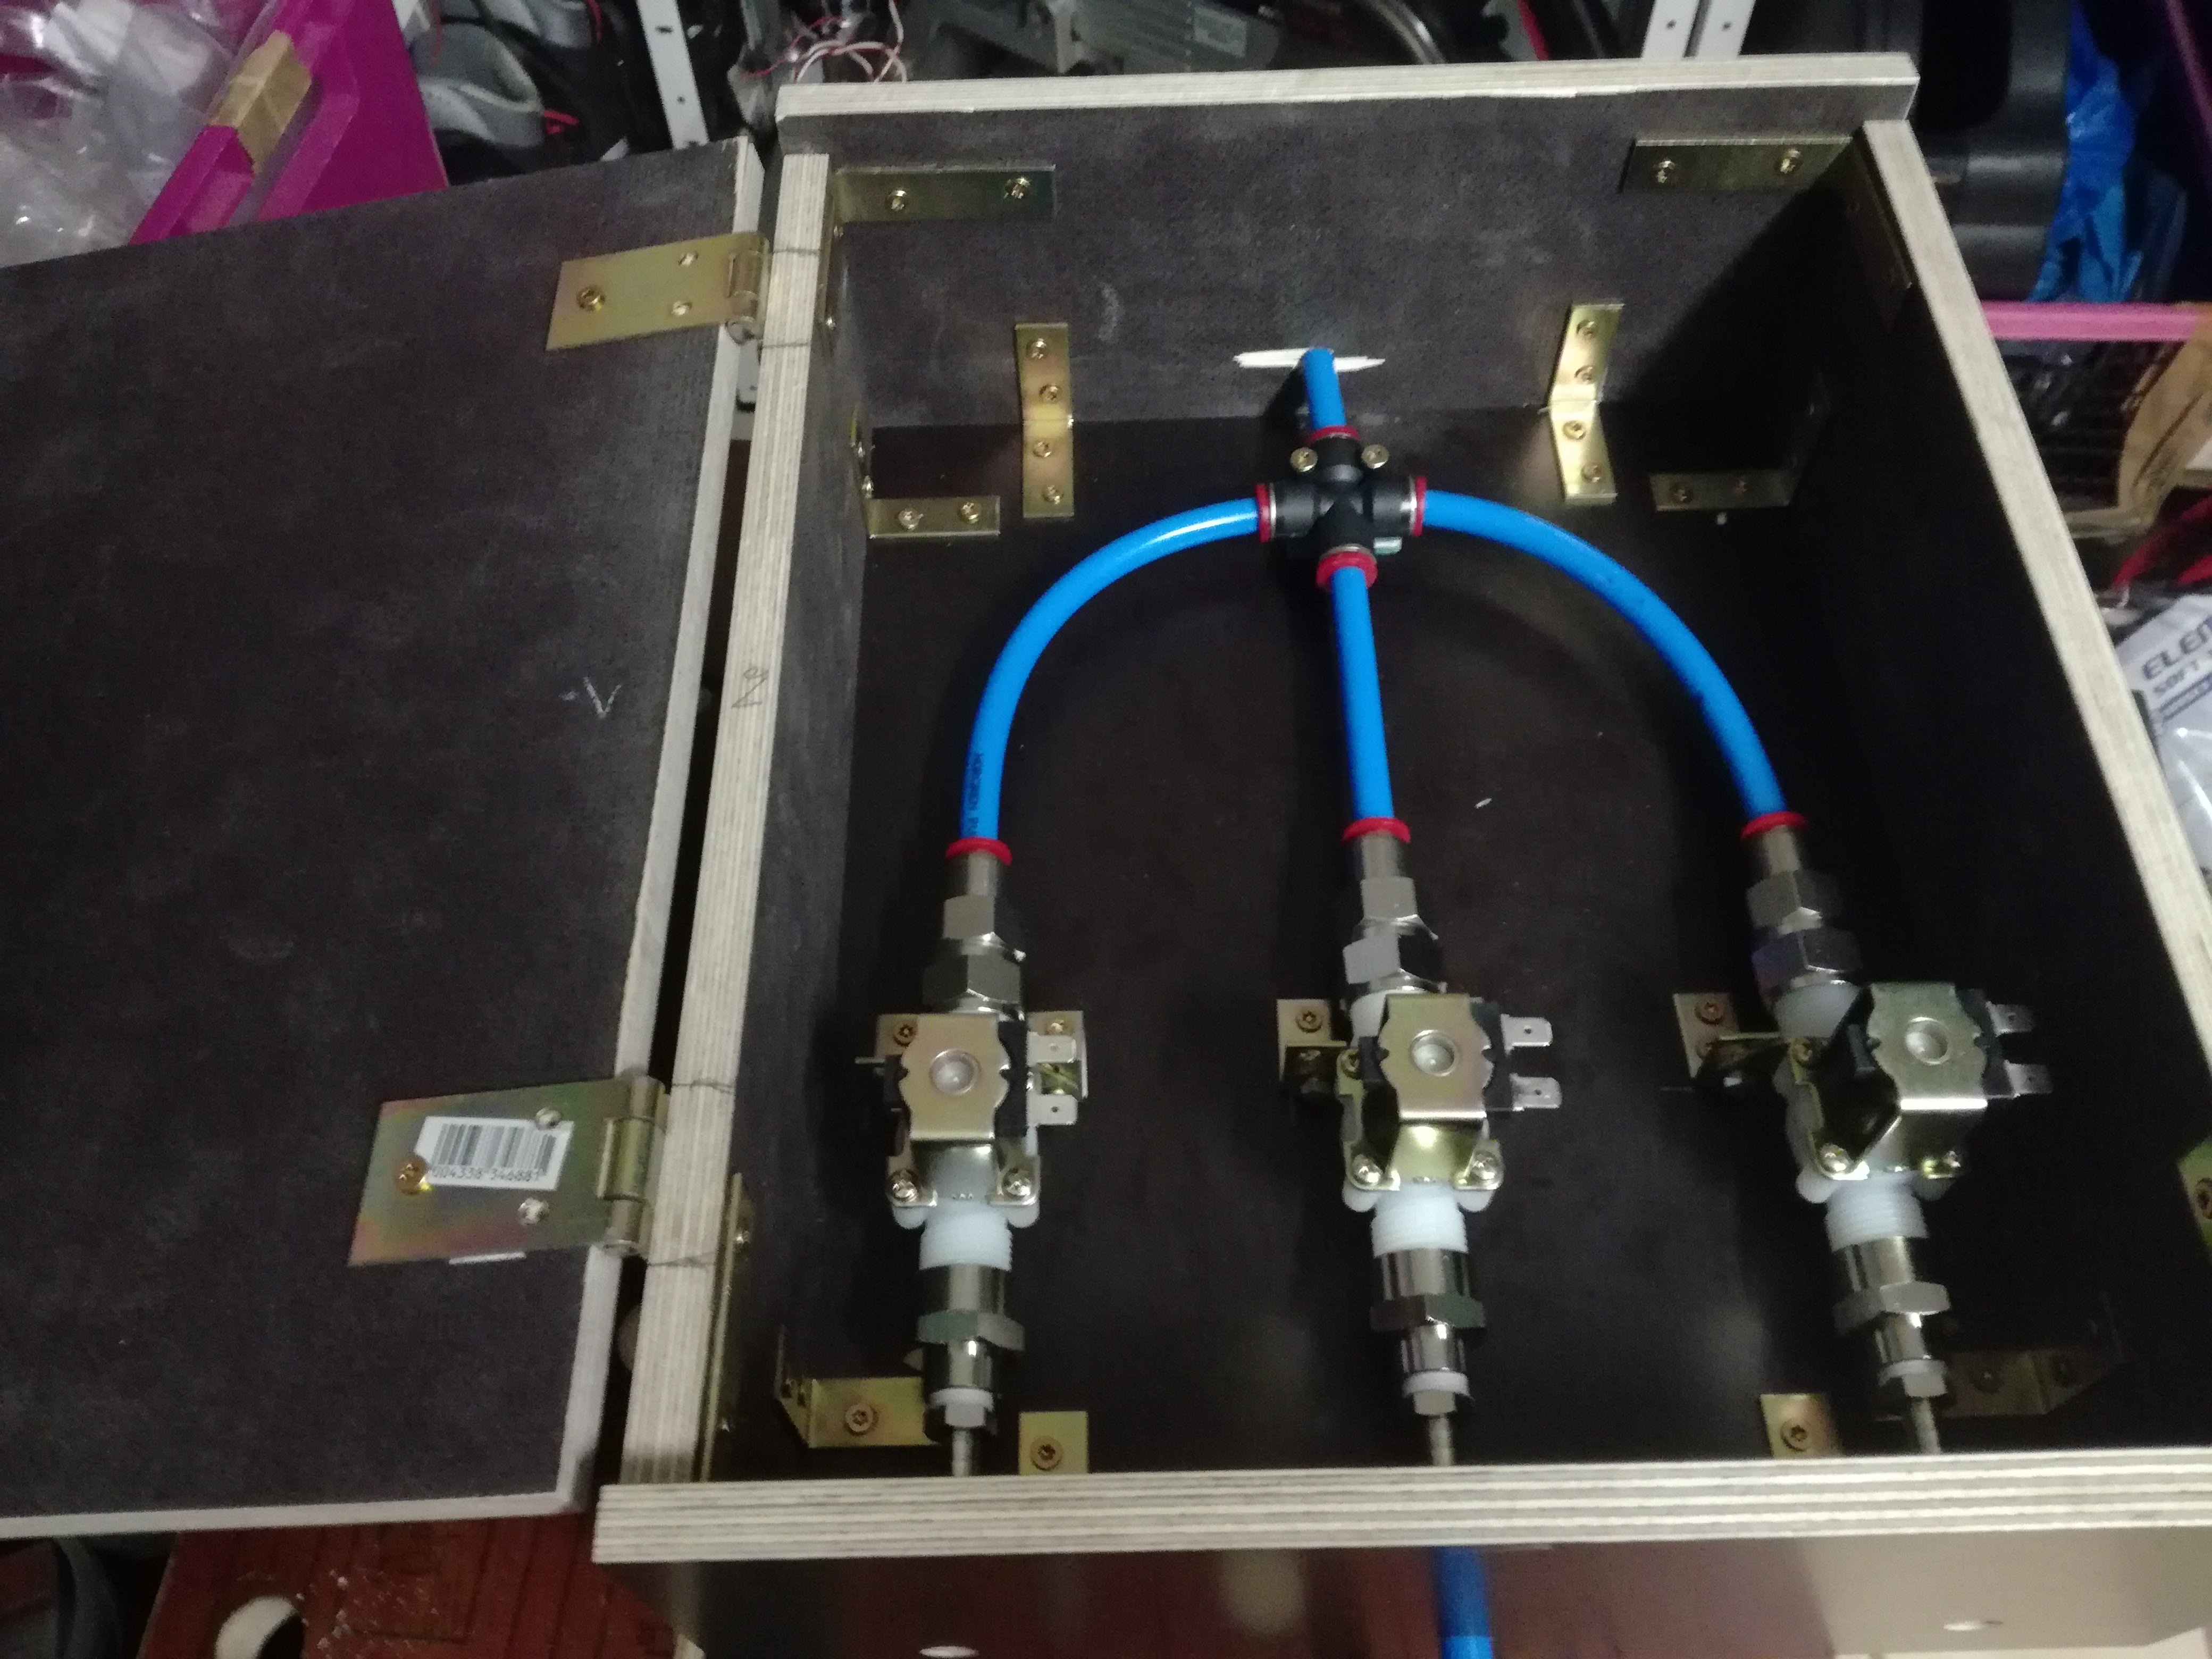
\includegraphics[width=\textwidth]{silas/gehause}
    \caption{Innenraum des Gehäuses}
\end{figure}
\newpage
\fancyhf{}
\lhead{Dennis Hufnagel}
\rhead{Seite \thepage}
\section{Feuchtigkeitssensor}
\subsection{Warum ein Feuchtigkeitssensor?}
Um das automatische Pflanzenbewässerungssystem zu realisieren, standen uns zwei
verschiedene Herangehensweisen zur Verfügung. Einerseits hätte man die Bewässerung nur
mit einem zeitbasierten Algorithmus durchführen können. Andererseits bestand die
Möglichkeit, als Basis für die Bewässerung auf Feuchtigkeitsmessungen zurückzugreifen.

\subsubsection{Nachteile/Vorteile einer rein zeitbasierten Bewässerung}
Ein großer Nachteil dieses Ansatzes ist, dass die Bewässerungsroutine zeitlich festgelegt ist.
So ist es praktisch unmöglich, auf sich verändernde Einflüsse in der Umgebung der Pflanze zu
reagieren. Eine Veränderung der Sonneinstrahlung, des Wetters und somit der
Luftfeuchtigkeit oder der Temperatur beeinflussen, wie schnell die Erde im Blumentopf
austrocknet. Während einer regnerischen und gleichzeitig kalten Jahreszeit, könnte die
Pflanze aufgrund der festen Bewässerungsroutine ertränkt werden, da die Erde während
eines Bewässerungsintervalls nicht stark genug trocknet. Dasselbe gilt natürlich auch
andersrum, dass die Pflanze während eines Intervalls zu stark austrocknet. Außerdem muss
für jede einzelne Pflanze ein individuelles Profil erstellt werden, da Pflanze unterschiedlich
viel Wasser benötigen. Somit besteht die Möglichkeit, dass die Pflanzen zu früh eingehen, da
nicht immer für optimale Bedingungen gesorgt werden konnte. Eine Option, dieses Problem
ohne Feuchtigkeitssensor zu beheben, wäre die Verwendung von Temperatursensoren und
die Miteinbeziehung von den lokalen Wetterdaten. So könnte man mit einer Kalkulation die
Zustände in der Erde und den Grad der Austrocknung approximieren. Dieses Verfahren ist
allerdings extrem umständlich und würde so den Rahmen dieser Projektarbeit sprengen.
Der Vorteil dieses Verfahrens ist seine Einfachheit bei der Anlegung der Routine. Zwar muss
für jede Pflanze eine eigene Erstellt werden, jedoch müssen keine Berechnungen oder
Messungen vorgenommen werden, um Sensoren zu kalibrieren und deren Daten mit dem
Feuchtigkeitsgrad der Erde zu korrelieren. Es muss lediglich die Routine programmiert
werden, damit das System einwandfrei funktioniert.

\subsubsection{Nachteile/Vorteile einer sensorbasierten Bewässerung}
Der größte Vorteil, der ein Feuchtigkeitssensor mit sich bringt, ist, dass der Zustand der Erde
gemessen werden kann. Somit können die äußeren Einflüsse ignoriert werden, da wir deren
Ergebnisse, die unterschiedlich schnell austrocknende Erde, messen können. Somit ist dieses
Verfahren flexibler und universeller anwendbar. Für unterschiedliche Pflanze müssen jetzt
keine individuellen Routinen programmiert werden, da Pflanzen, die z.B. weniger Wasser
benötigen, die Erde einfach langsamer austrocknen. So müssen nur die Daten ausgelesen
werden und daraufhin kann dann entschieden werden, ob gewässert werden muss oder
nicht.
Ein Nachteil dieser Technik ist die Notwendigkeit, Sensoren zu entwickeln und immer für die
unterschiedlichen Erden zu kalibrieren. Dies ist wichtig, damit der Sensor eine trockene Erde
auch als solche ausliest. Letztendlich ist dieser Ansatz jedoch der Effizientere.

\subsection{Entwurf des Feuchtigkeitssensors}
\subsubsection{Theorie des Sensors} \label{sensortheorie}
Zuallererst musste entschieden werden, ob fertige Sensoren gekauft werden, oder der
Sensor selber entwickelt wird. Da wir zu viert an dieser Projektarbeit gearbeitet haben,
konnten die Sensoren selber entwickelt werden, da genug Ressourcen vorhanden waren.
Nachdem dies geklärt war, musste eine Entscheidung zwischen der kapazitiven und der
resistiven Messmethode getroffen werden. Aufgrund der Probleme durch die mögliche
Elektrolyse in der Erde, wurde sich für die kapazitive Messmethode entschieden.
Die Formel um die Größe eines Kondensators zu bestimmen, lautet:
\begin{center}
    $C = \varepsilon _R * \varepsilon _0 * \frac{A}{d}$ (1)
\end{center}
Wobei $A$ der Fläche der Kondensatorplatten, $d$ dem Abstand zwischen den Platten, $\varepsilon _0$ der
elektrischen Feldkonstante und $\varepsilon _R$ der Permittivitätszahl entspricht. Das Prinzip der
kapazitiven Messmethode beruht darauf, dass sich mit einer Änderung der Feuchtigkeit auch
die Permittivitätszahl verändert. Da $\varepsilon _0$ eine Konstante ist und der geometrische Aufbau des
Sensors und somit des Kondensators sich nicht verändert, bleiben $A$ und $d$ auch konstant.
Somit ist die Größenveränderung des Kondensators ausschließlich von der sich ändernden
Permittivitätszahl abhängig.

\subsubsection{Schaltplan/Funktion des Sensors}
Nun musste die Schaltung für solch einen Sensor entwickelt werden. Dazu wurde im Internet
recherchiert und Konkurrenzprodukte analysiert. Letztendlich wurde sich dafür entschieden,
einen Schmitt-Trigger mit Hysterese zu verwenden. Die Hysterese dient dazu, den Schmitt-Trigger
weniger anfällig gegen Störungen zu machen. Hiermit lässt sich ein recht einfacher,
jedoch akkurater Sensor bauen.
\begin{figure}[ht]
    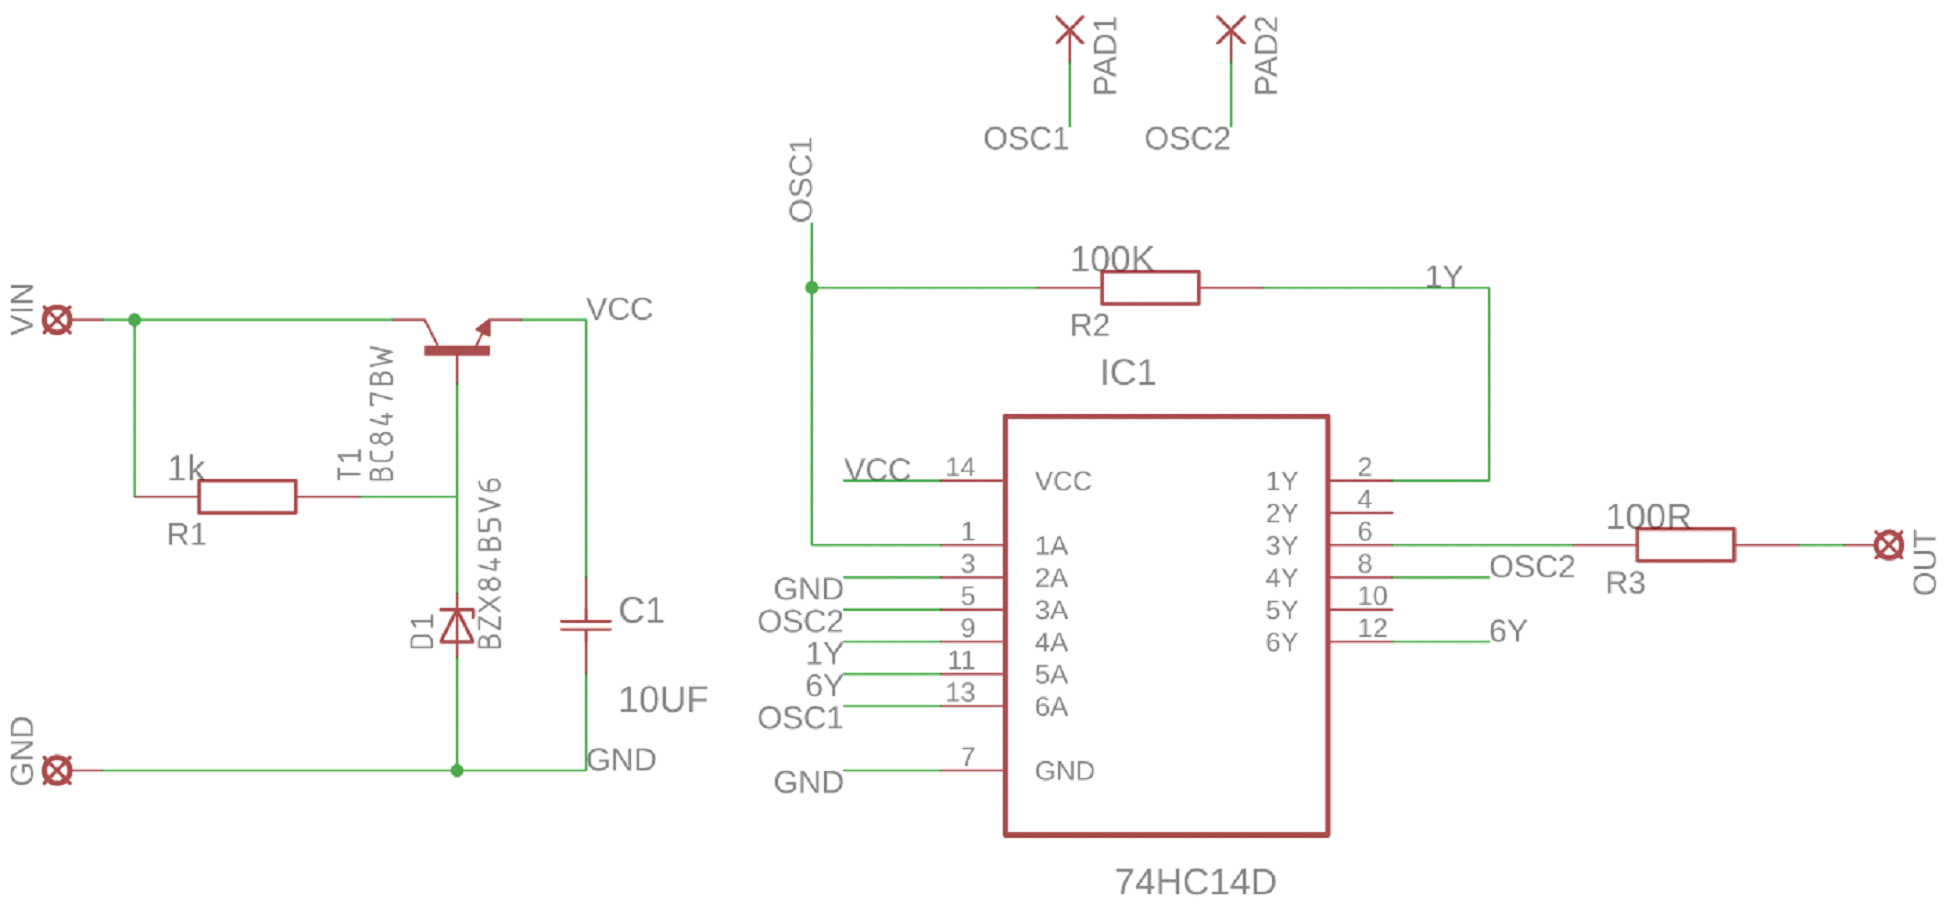
\includegraphics[width=\textwidth]{dennis/schaltplan}
    \caption{Schaltplan des Feuchtigkeissensors}
\end{figure}

Der $IC1$ besitzt bis zu sechs invertierende Schmitt-Trigger, welche jeweils von ihrem Eingang
$A$ bis zum Ausgang $Y$ verbaut sind. Versorgt wird er mit einer Gleichspannung von $5V$. Diese
wird von dem linken Teil der Schaltung erzeugt. Diese kleine Konstantan-Spannungsquelle
wurde eingefügt, da wir zu Beginn noch nicht wussten, mit welcher Spannung wir den Sensor
versorgen können. Der Schmitt-Trigger, der wichtig für unsere Schaltung ist, ist an seinem
Eingang 1A mit einer Kondensatorplatte OSC1 verbunden. Die Hysterese ist über den $100k\Omega$
Widerstand mit dem Ausgang $1Y$ verbunden. Die zweite Kondensatorplatte ist an dem
Schmitt-Trigger Eingang $3A$ angeschlossen. Der Ausgang $3Y$ ist noch mit einem $100\Omega$
Widerstand belastet, damit ein etwas höherer Strom durch die Leitungen fließt. Die anderen
Anschlüsse am I$C1$ als die oben genannten, dienen nur dem Zweck, das routen der
Leiterbahnen zu vereinfachen. Sie haben keinen Einfluss auf die Funktionalität der Schaltung.
Da der Schmitt-Trigger invertierend ist, lädt er, solange die Schaltschwelle noch nicht
erreicht ist, den Kondensator über den Widerstand auf. Diese erste Kondensatorplatte $OSC1$
lädt somit die zweite Platte $OSC2$ auf. Erreicht die zweite Kondensatorplatte somit die
Schwellenspannung, wechselt der Schmitt-Trigger an seinem Ausgang $3Y$ von 1 auf 0 und
entlädt die Kondensatorplatte $OSC2$ dabei. Nun beginnt dasselbe Prinzip wieder von vorne.
$OSC2$ wird wieder aufgeladen und der Schmitt-Trigger wechselt beim Erreichen seiner
Schwellenspannung wieder von 1 auf 0. Da die Zeit, die benötigt wird um den Kondensator
aufzuladen, abhängig von dessen Größe ist, haben wir eine variable Frequenz, die von der
Größe des Kondensators abhängig ist. Da wir unter Kapitel \ref{sensortheorie} gelernt haben
, dass die Größe des Kondensators nur von der Permittivitätszahl abhängig ist, bedeutet das, dass die
Frequenz, mit der unser Schmitt-Trigger schaltet, von der Permittivitätszahl und somit von
dem Feuchtigkeitsgrad der Erde abhängig ist. Je trockener die Erde, desto kleiner wird die
Permittivitätszahl und somit der Kondensator. Somit liefert der Sensor bei trockener Erde
eine höhere Frequenz als bei nasser, da der Kondensator schneller aufgeladen wird. Der
Verlauf der Frequenz in Abhängigkeit von dem Feuchtigkeitsgrad der Erde verläuft linear.
Somit haben wir am $OUT$ Ausgang unsere Schaltung ein $5V$ Signal mit variierender Frequenz
anliegen, welches wir mit dem Arduino UNO auslesen können.
Das Erstellen des Platinenlayouts des Sensors wird im Kapitel \ref{sensorlayout} beschrieben.

\subsubsection{Messergebnisse des Sensors}
Nachdem das Layout des Sensors fertiggestellt wurde (Kap. \ref{sensorlayout}), konnte die Platine mit der
Ätzmaschine der Hochschule geätzt werden. Danach konnten auf jedem Sensor die Bauteile
aufgebracht und festgelötet werden. Damit sichergestellt werden kann, dass jeder Sensor
problemlos funktioniert und alle Lötstellen korrekt angebracht wurden, muss jeder Sensor
einem Funktionstest unterzogen werden. Dazu wird jeder einzelne Sensoren an $+5V$ und das
$OUT$-Signal an ein Oszilloskop angeschlossen. Der Sensor wurde dann zuerst an der Luft
getestet, um seine korrekte Funktionsweise zu überprüfen. War dies Erfolgreich, wurde der
Sensor mit dem Schutzlack Plastik 70 eingesprüht, um die Platine vor Korrosion zu schützen.
Danach wurde der Sensor in einen kleinen Behälter mit Erde gesteckt. Diese war kaum mit
Wasser angesetzt, um den Sensor in trockenen Verhältnissen zu testen.
\begin{figure}[ht]
    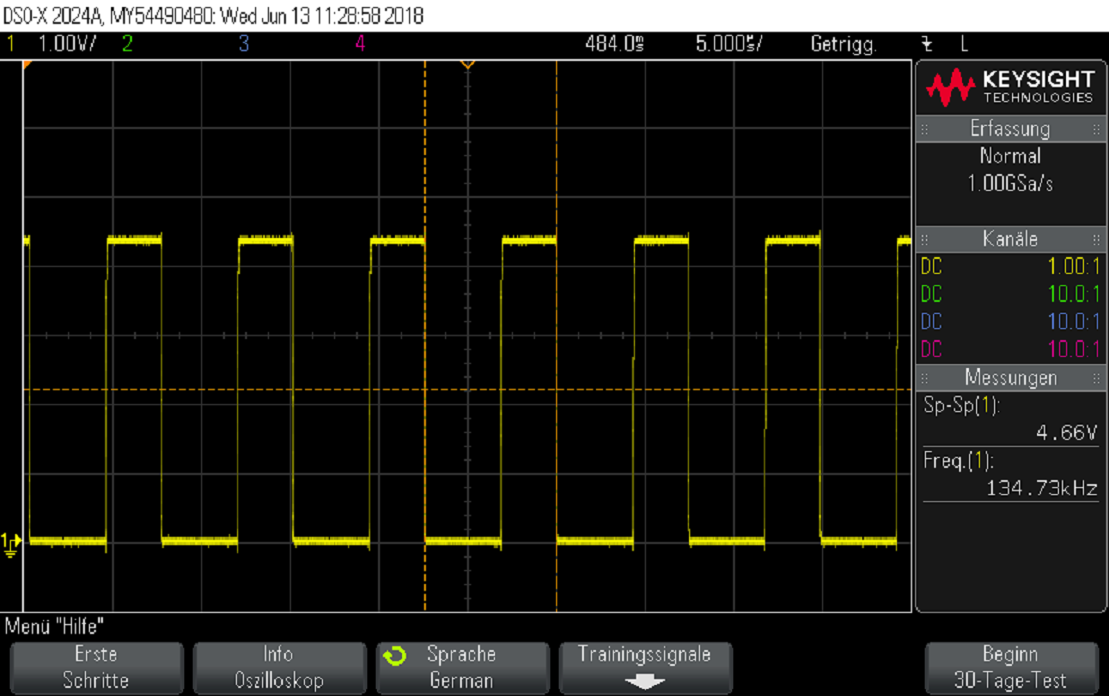
\includegraphics[width=\textwidth]{dennis/trocken}
    \caption{Auslesen des Sensors bei trockener Erde}
\end{figure}
Dann wurde etwas Wasser in die Erde gegossen und, wie zu erwartend, eine Verringerung der
Frequenz festgestellt.
Somit konnte die korrekte Funktionsweise jedes Sensors bewiesen werden.
\begin{figure}[ht]
    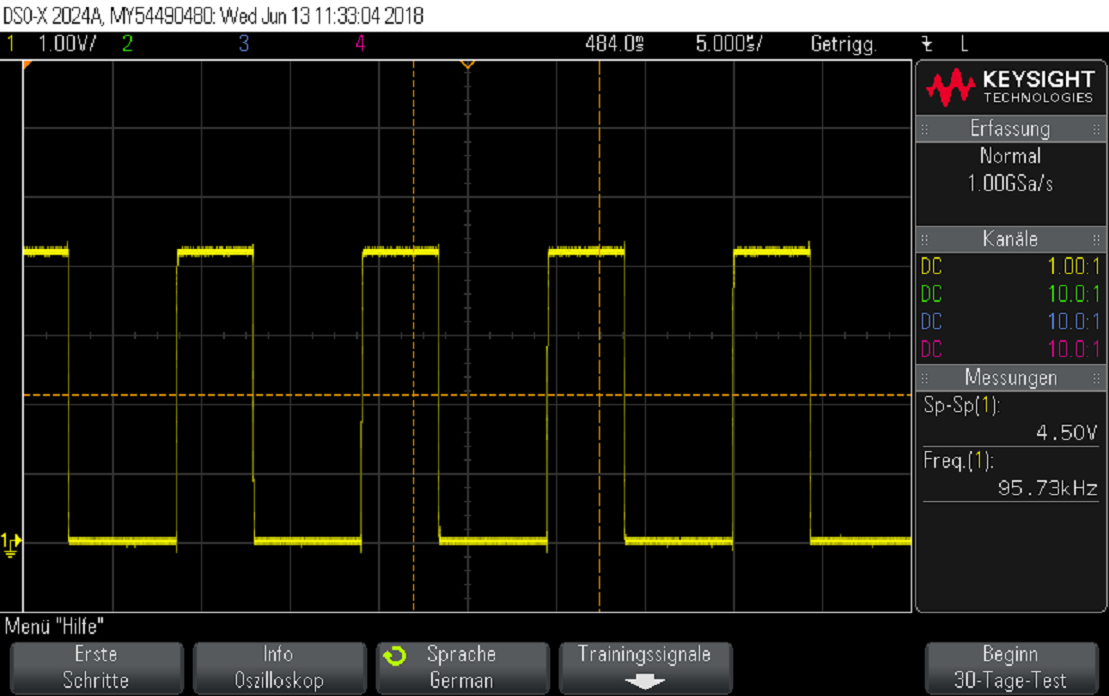
\includegraphics[width=\textwidth]{dennis/feucht}
    \caption{Auslesen des Sensors bei feuchter Erde}
\end{figure}

\section{Erstellen der Platinenlayouts}
\subsection{Layout des Feuchtigkeitssensors} \label{sensorlayout}
Bevor damit begonnen werden konnte, den Sensor in Eagle zu routen, musste festgelegt
werden, inwiefern der Sensor aufgebaut wird. Der Aufbau eines normalen Kondensators
besteht aus zwei gegenüberliegenden Platten (Abbildung \ref{fig:kond1}). Dieser Aufbau würde sich
allerdings als relativ umständlich erweisen, da man somit den Sensor in drei einzelne
Platinen aufteilen müsste. Je zwei für die zwei Kondensatorenplatte und die dritte Platine für
die Elektronik. Diese Platinen müsste man noch über Winkel dann miteinander fixieren,
damit der Abstand der Kondensatorplatten zueinander auch konstant bleibt. Da dieser
Aufbau somit zu umständlich war, wurde nach Alternativen gesucht. Das Ergebnis ist, dass
die beiden Kondensatorplatten jetzt nebeneinander, anstatt übereinander, angelegt werden.
Dies wird in Abbildung \ref{fig:kond2} verdeutlicht.
\begin{figure}[ht]
    \centering
    \begin{minipage}{0.45\textwidth}
        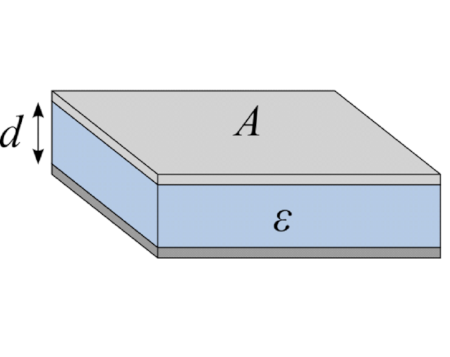
\includegraphics[width=0.9\textwidth]{dennis/kond1}
        \caption{Kondensatorplatten übereinander}
        \label{fig:kond1}
    \end{minipage}
    \begin{minipage}{0.45\textwidth}
        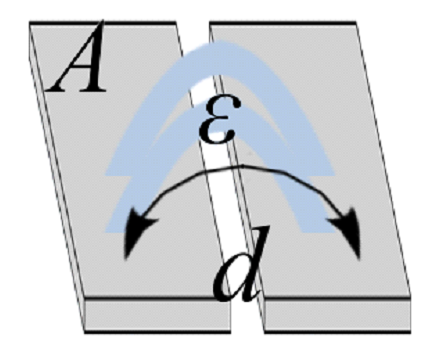
\includegraphics[width=0.9\textwidth]{dennis/kond2}
        \caption{Kondensatorplatten nebeneinander}
        \label{fig:kond2}
    \end{minipage}
\end{figure}
Ein Problem dieses Ansatzes ist allerdings, dass sich die Geometrie ändert und somit die
Formel (1) nicht mehr stimmt. Da allerdings, wie unter Kapitel \ref{sensortheorie} beschrieben, die
Geometrie konstant bleibt, ist die Änderung der Kondensatorgröße weiterhin nur von der
Permittivitätszahl abhängig. Die veränderte Geometrie spielt somit für die Funktion der
Schaltung keine Rolle. Nun konnte mit dem Anlegen des Platinenlayouts begonnen werden.
\begin{figure}[h]
    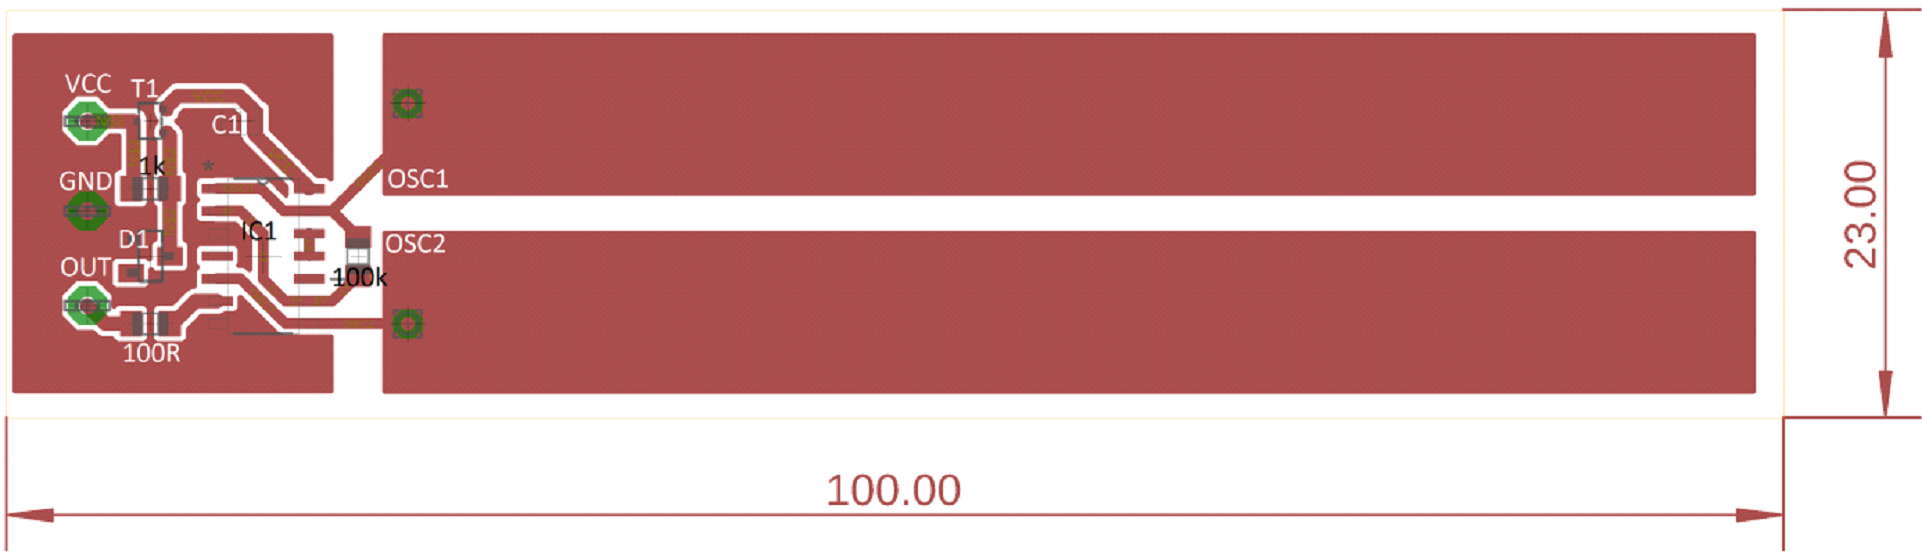
\includegraphics[width=\textwidth]{dennis/layout2}
    \caption{Layout des Feuchtigkeissensors}
\end{figure}
Die elektronischen Bauteile wurden auf der linken Seite angeordnet. Während die beiden
großen Kupferpolygone auf der rechten Seite die Kondensatorplatten repräsentieren. Somit
kann der Sensor in die Erde gesteckt werden, ohne dass die Bauteile mit der Erde in Kontakt
treten müssen. Generell wurden die Bauteile so kompakt wie möglich angeordnet, damit die
Platine am Ende nicht zu groß wird. Der Sensor muss natürlich in jeden Blumentopf passen.
Die drei Anschlüsse der Platine ($VCC$, $GND$, $OUT$) wurden für eine gute Erreichbarkeit, ganz
am Rand angebracht. Dadurch müssen auch die Kabel nicht durch die Erde geführt werden.
Für einen besseren Anschluss der $GND$-Pins der Bauteile, wurde ein $GND$-Polygon um die
Bauteile herum angebracht. Dadurch wird der Stromfluss des $GND$-Potentials verbessert. Die
restlichen Verbindungen wurden dann, je nach Möglichkeit, mit einer möglichst breiten
Leiterbahn verbunden. Eine breitere Leiterbahn verbessert den Stromfluss.

\subsection{Layout der Leistungsschaltungsplatine}
\begin{figure}[h]
    \centering
    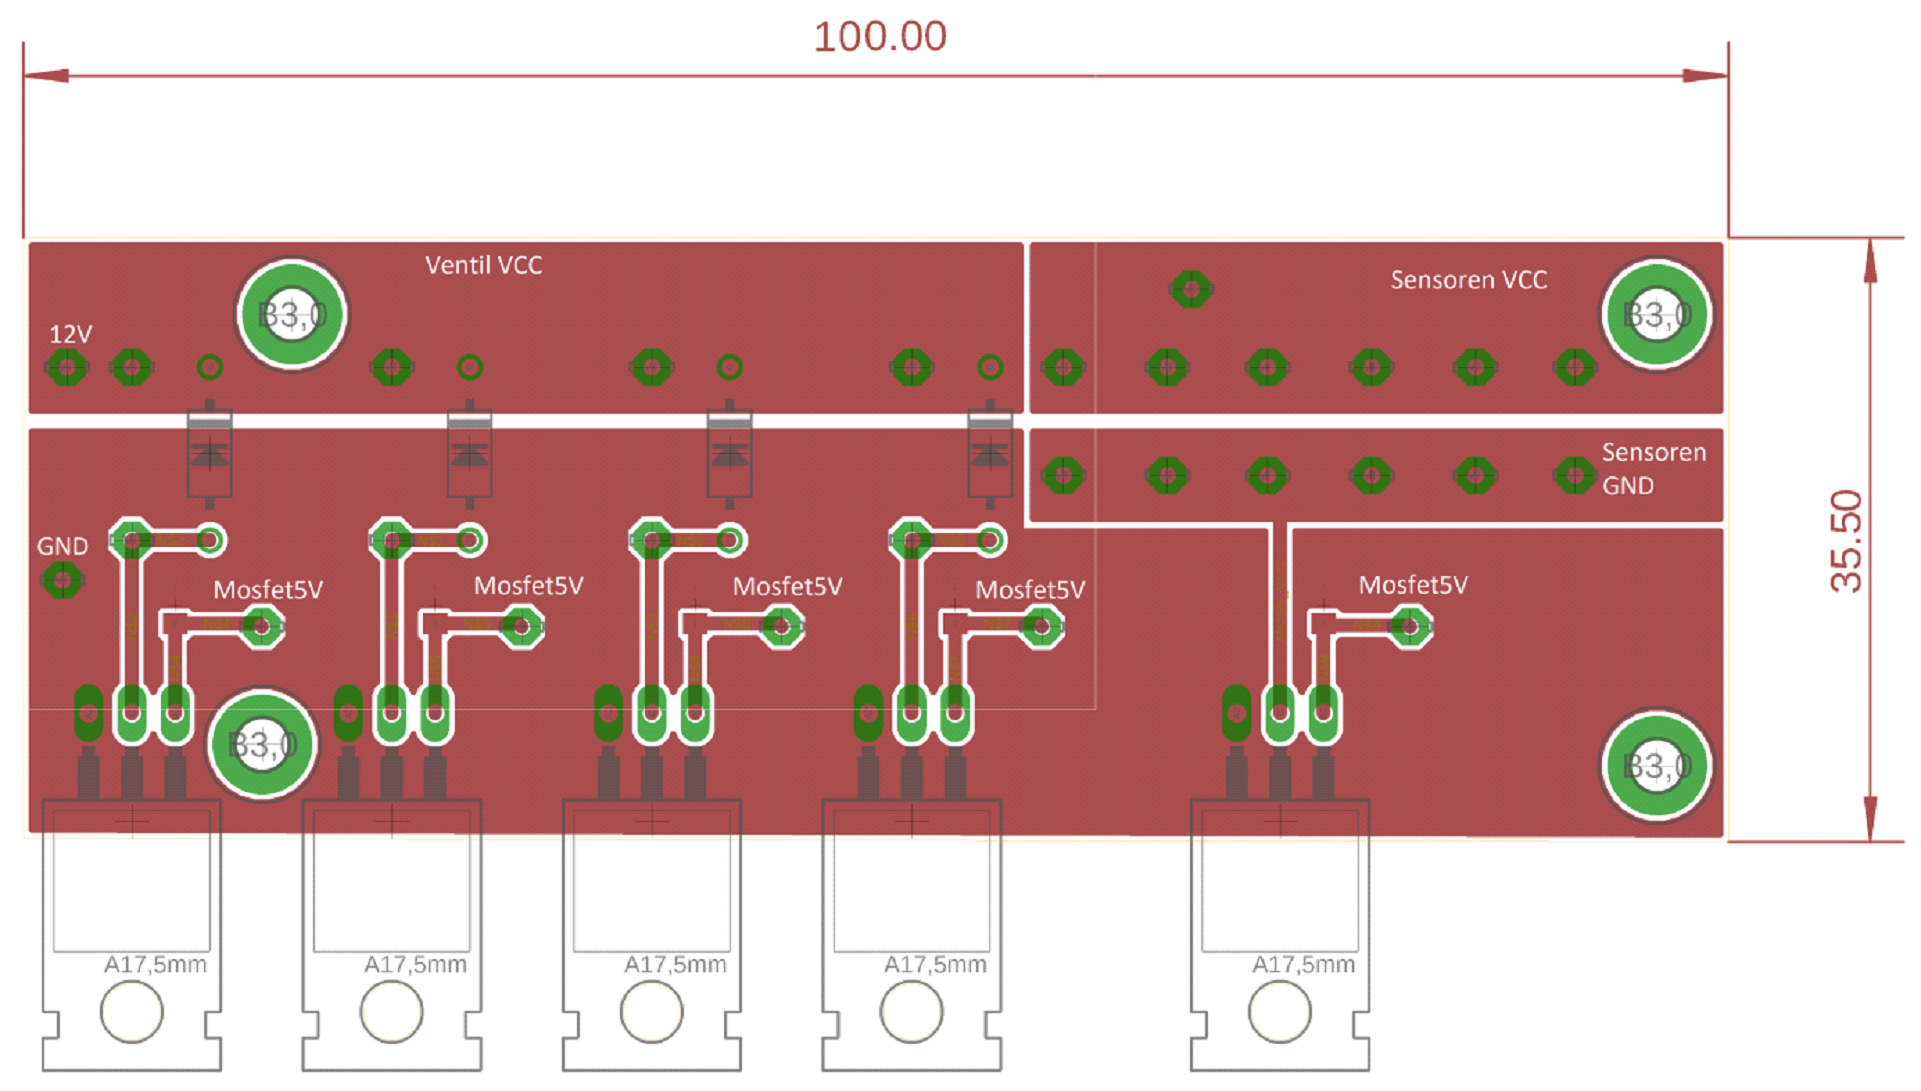
\includegraphics[width=\textwidth]{dennis/layout1}
    \caption{Layout der Leistungsschaltungsplatine}
\end{figure}

Die Ventile, die wir verwenden, benötigen $12V$ Versorgungsspannung und bis zu $300mA$
Strom. Dies kann der Arduino selbstverständlich nicht leisten. Deswegen musste eine
weitere Platine entworfen werden, die die Ansteuerung und Versorgung der Ventile, der
Pumpe und auch die Versorgung der Sensoren übernimmt. Der Entwurf der Schaltung und
die Entwicklung des Schaltplans hat mein Kollege Silas Leidel übernommen. Von mir wurde
dann noch das Layout angefertigt, da ich bereits Erfahrung damit hatte. Zur Steuerung der
Ventile, Sensoren und Pumpe wurde an jeden Anschluss ein MOSFET hinzugefügt. Die Pfade
für die Pumpe und die Ventile besitzen auch noch eine dazu parallele Rücklaufdiode. Die VCC
Anschlüsse der Ventile und Pumpen werden im linken, oberen $12V$ Polygon
angeschlossen. Ihr $GND$ Anschluss wird dann links, neben den Dioden VIA verlötet. Am
unteren Ende der Platine sitzt der MOSFET, der wiederum von dem Arduino über den
Mosfet $5V$ Anschluss gesteuert wird. Diese Anordnung existiert insgesamt viermal, dreimal
für die drei Ventile und einmal für die Pumpe. Da die Sensoren mit $5V$ versorgt werden,
musste für sie ein extra Polygon zur Stromversorgung angelegt werden. Versorgt wird dieses
Potential von der unter Kapitel \ref{stromlayout} vorgestellten Platine. Es wurde entschieden,
nur einen MOSFET für alle Sensoren zu verwenden, da sonst die Platine, wegen der
zusätzlichen MOSFET, zu groß geworden wäre. Um den Stromfluss zu verbessern, wurden
wieder alle Spannungspotentiale als Polygon realisiert. Am Ende wurden noch vier M3
Befestigungslöcher hinzugefügt, damit die Platine einfacher an einem Gehäuse befestigt
werden kann.

\subsection{Layout des Stromverteilers} \label{stromlayout}
\begin{figure}[h]
    \centering
    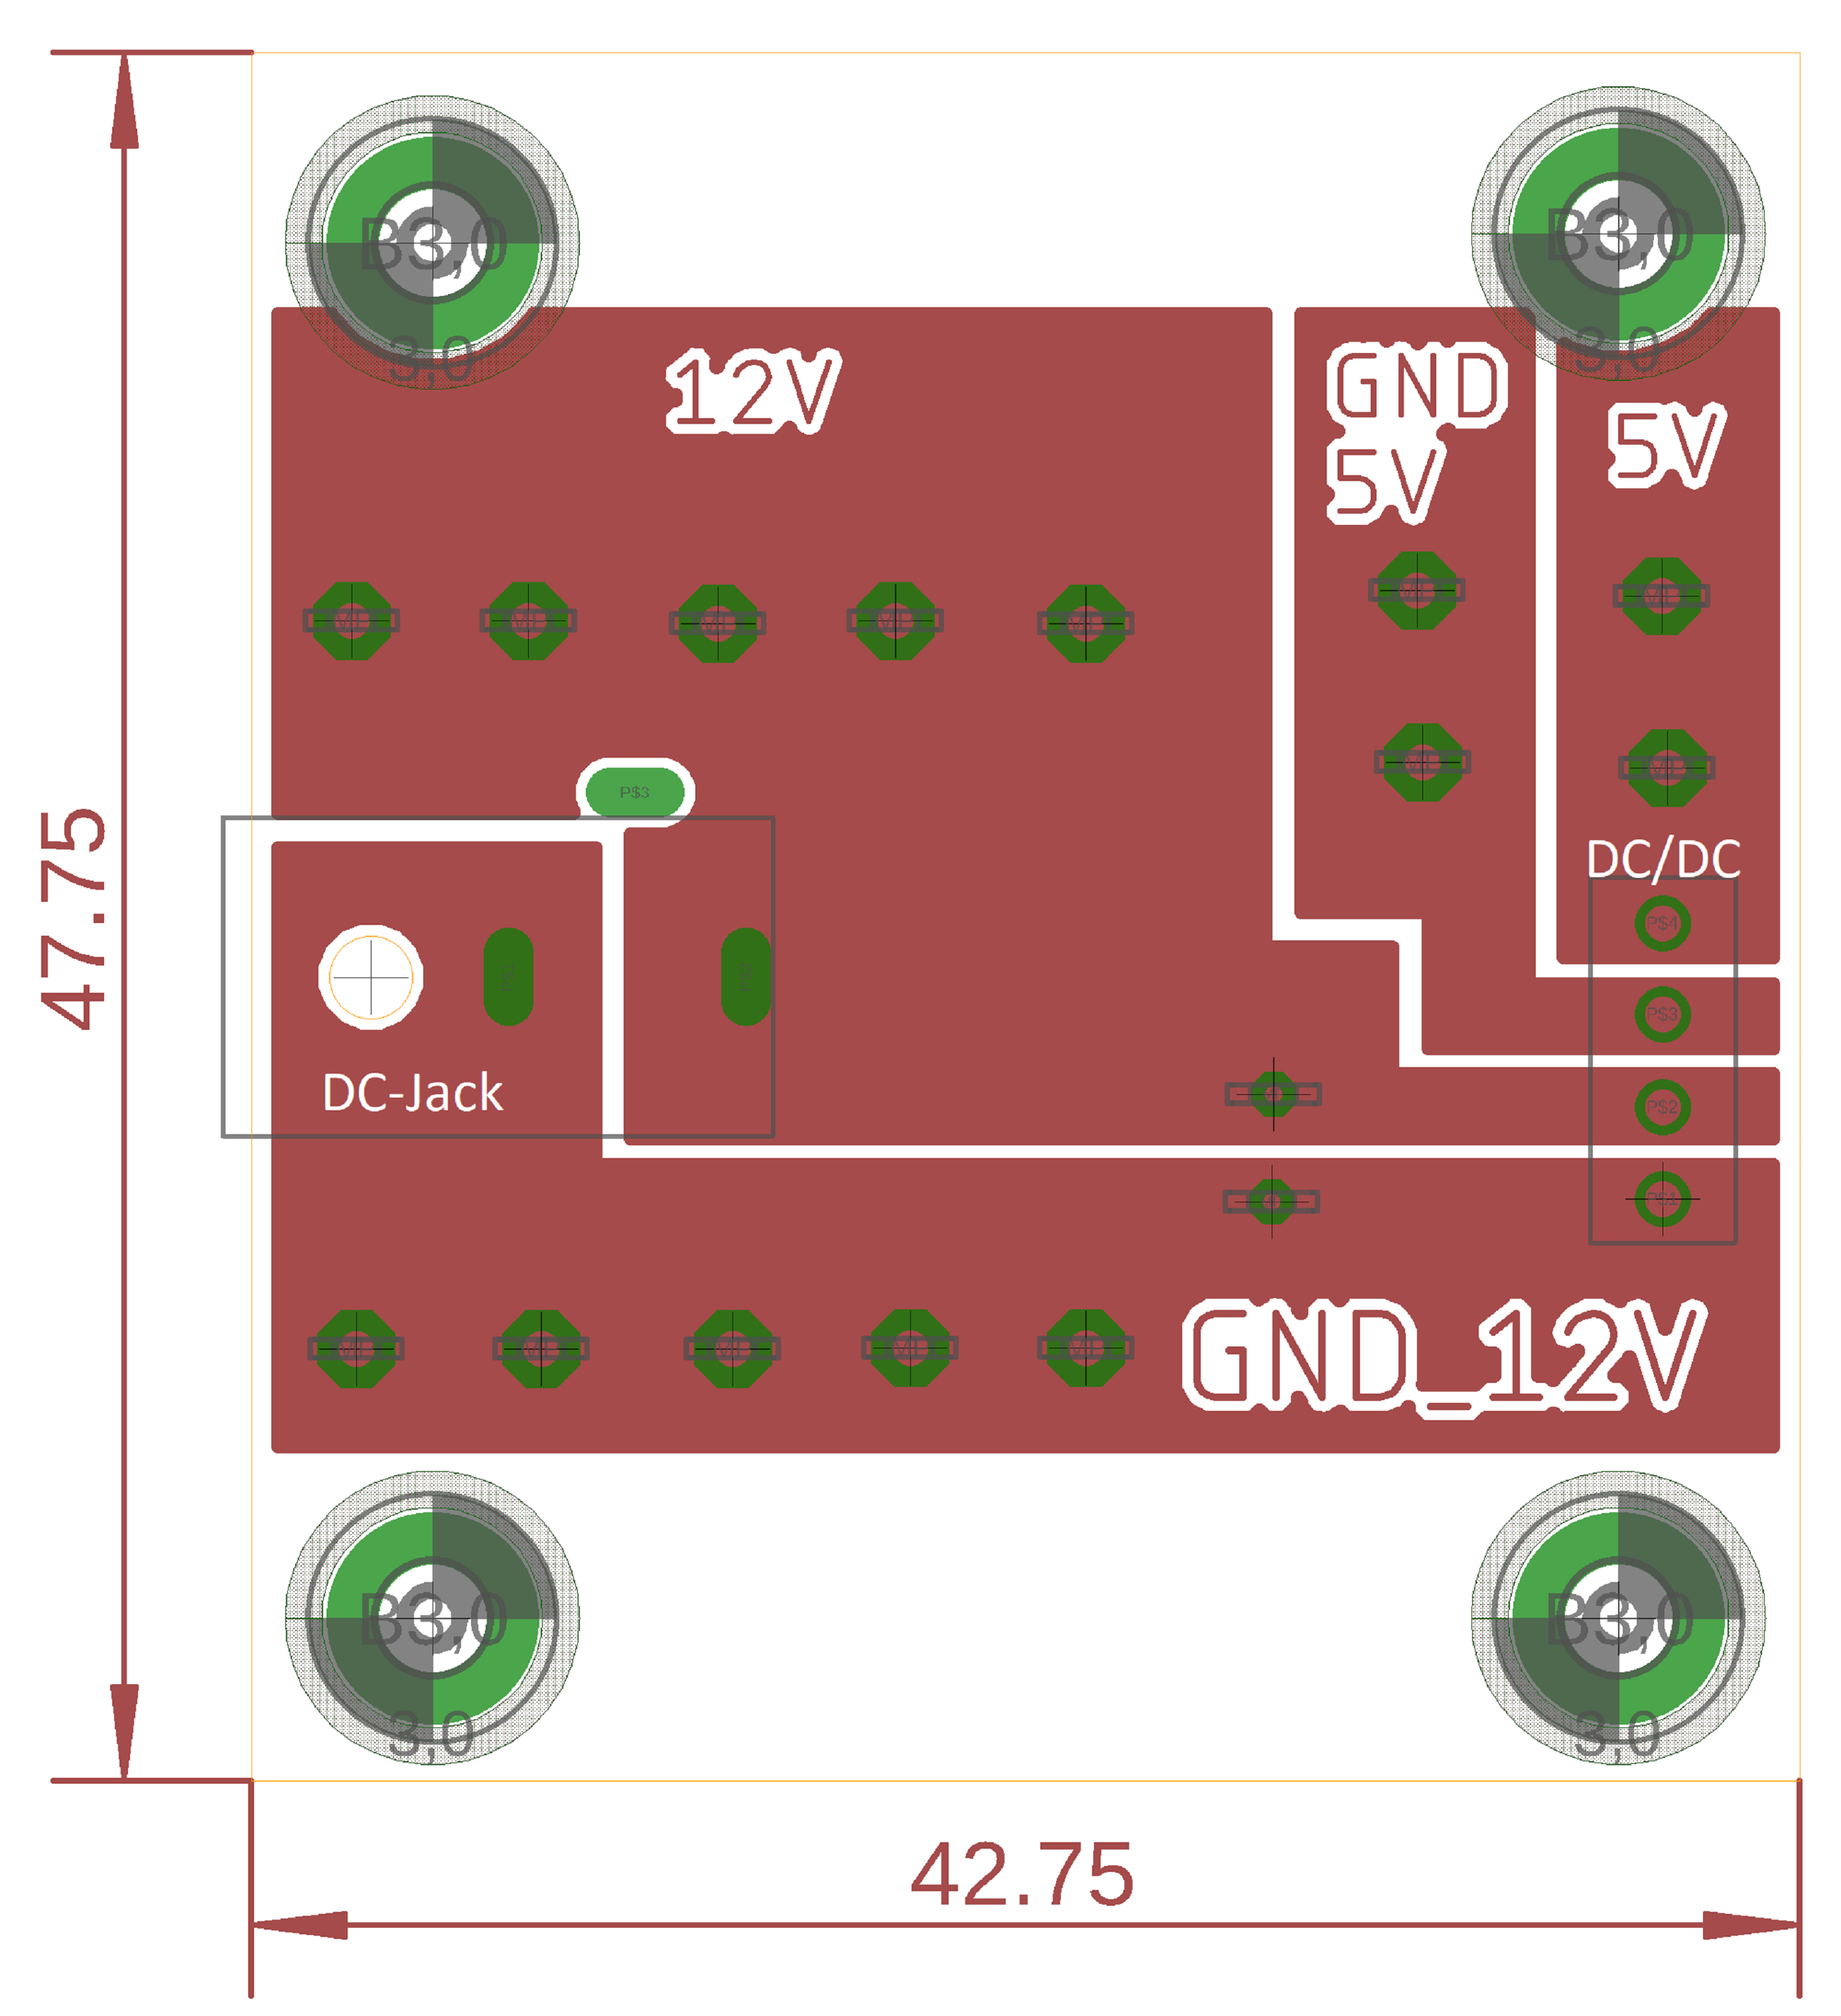
\includegraphics[width=0.5\textwidth]{dennis/layout}
    \caption{Layout der Stromverteilers}
\end{figure}
Diese Platine dient als Stromverteiler bzw. Stromwandler für unsere Elektronik. Die Sensoren
benötigen $5V$ Versorgungsspannung, während der Arduino, die Ventile und die Pumpe $12V$
brauchen. Das verwendete, externe Netzteil kann allerdings nur $12V$ liefern. Damit wir diese
$12V$ einerseits auf die verschiedenen Platinen und Bauteile verteilen können und
andererseits auf $5V$ umwandeln können, wurde diese Platine entworfen. Die Schaltung
stammt wieder von meinem Kollegen Silas Leidel. Der DC-Jack ist der Anschlussstecker an
das externe Netzteil, dass die 230V Wechsel- auf $12V$ Gleichspannung transformiert. Diese
$12V$ werden dann mit dem DC/DC Konverter auf $5V$ heruntertransformiert. Diese $5V$ dienen
dann als Versorgungsspannung für die Sensoren. Die verschiedenen Spannungspotentiale
sind auch hier wieder als Polygone ausgeführt. Letztendlich wurden der Platine noch vier M3
Bohrlöcher hinzugefügt, um ihre Befestigung am Gehäuse zu vereinfachen. Das Verlöten des
DC-Jack erwies sich jedoch in der Praxis als schwierig. Hierfür wäre es einfacher gewesen,
Polygone auf der Vorder- und Rückseite zu verwenden und diese mittels VIAs zu verbinden.
\newpage
\fancyhf{}
\lhead{Marcel Fuchs}
\rhead{Seite \thepage}
\section{Software - Arduino}
\subsection{Allgemeines}
Für Umsetzung der automatischen Steuerung des Systems wurde, wie bereits erläutert
auf ein Arduino Mikrocontrollerboard gesetzt. Die Programmierung erfolgt über den
bordeigenen Bootloader wodurch kein externer Programmer oder Debugger nötig ist. Des
Weiteren wurde das gesamte Softwareprojekt in der Arduinoeigenen IDE erstellt und editiert.
\subsection{Objektorientierung}
Da das Bewässerungssystem für mehrere Pflanzen geeignet sein soll und man somit
mehrere Aktoren mit denselben Funktionen hat ist es sinnvoll diesen Teil des Software
Projektes Objektorientiert zu gestalten. Die Objektorientierung bietet außerdem den
Vorteil ohne viel Aufwand weitere Pflanzen mit dem System zu bewässern.
\begin{figure}[ht]
    \centering
    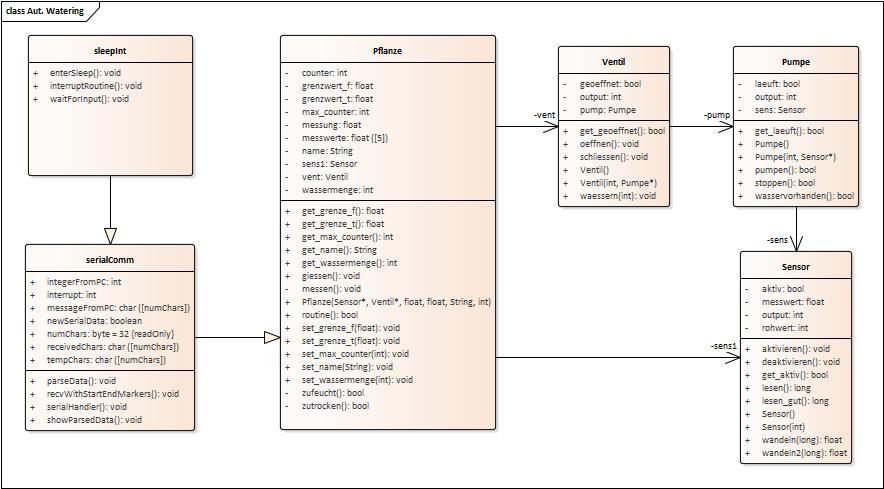
\includegraphics[width=\textwidth]{marcel/AutWatering}
    \caption{Klassendiagramm des Programms auf dem Arduino}
    \label{arduinoklassen}
\end{figure}

So gibt es für jede zu bewässernde Pflanze ein Objekt der Klasse Pflanze. Wie in
Abbildung \ref{arduinoklassen} zu sehen beinhaltet diese Informationen zu allen wichtigen Kenndaten.
So werden ihr Feuchtegrenzwerte, die Wassermenge pro Wässerung, ein Name und die
übliche Zeit zwischen zwei Wässerungen zugewiesen. Außerdem werden das zugehörige
Ventil und der passende Sensor referenziert. Um diese Attribute auch während des
Programmablaufes ändern oder auslesen zu können gibt es diverse „get-“ und „set-“
Funktionen.  Die Datenverarbeitung und Signalerzeugung wird von den restlichen
Funktionen übernommen.
Für den angesprochenen Sensor und Ventil ist ebenfalls je eine Klasse implementiert.
Entscheidend sind hier die Attribute In- bzw. Output. Diese verweisen auf je einen
digitalen GPIO Pin des Arduino Boards. An diesen ist die jeweilige Steuerelektronik
angeschlossen, sodass man über diese Ports das Ventil steuern und den Sensorwert
auslesen kann. Die Funktionen übernehmen wieder den Teil der Datenverarbeitung und
Singalerzeugung. Eine letzte Klasse stellt die Pumpe dar. Von dieser Klasse wird nur
ein Objekt erzeugt, das von jedem Ventilobjekt referenziert wird. Eine kurze
Beschreibung der Funktionen finden sie in der folgenden Tabelle:
\hbadness=10001
\begin{tabular}{|l|p{0.55\textwidth}|}
    \hline
    Name der Funktion &	Funktionsbeschreibung\\ \hline
    Pumpe::pumpen() &	Setzt den Pin High an dem die Pumpe angeschlossen ist, wenn Wasser vorhanden ist.\\ \hline
    Pumpe::stoppen() &	Setzt den Pin Low an dem die Pumpe angeschlossen sit.\\ \hline
    Pumpe::wasservorhanden() &	True: Wenn Wasserstandsensor $< 250kHz$ liefert\\ \hline
    Ventil::oeffnen() &	Setzt Ventil-Pin high\\ \hline
    Ventil::schliessen() &	Setzt Ventil-Pin low\\ \hline
    Ventil::waessern(int dauer) & Startet Pumpe; Öffnet nach fester Verzögerung Ventil; Nach gegebener Dauer wird Ventil und Pumpe geschlossen.\\ \hline
    Pflanze::giessen() &	Pflanze wird gegossen (Ventil::waessern) und Zähler zurückgesetzt.\\ \hline
    Pflanze::zufeucht() &	Basierend auf aktueller und letzten Messungen wird entschieden, ob die Pflanze zu feucht ist.\\ \hline
    Pflanze::zutrocken() &	Basierend auf aktueller und letzten Messungen wird entschieden, ob die Pflanze zu trocken ist.\\ \hline
    Pflanze::routine() &	Aktuelle Feuchte wird gemessen, gespeichert und aufgrund des Wässerungsalgorithmus entschieden, ob die Pflanze nun gegossen wird\\ \hline
    Sensor::lesen() &	Sensor ließt die Frequenz an den zugewiesenen Inputport\\ \hline
    Sensor::wandeln() &	Die gelesene Freuqenz wird in einen prozentualen Feuchtewert gewandelt\\ \hline
\end{tabular}


\newpage
\subsection{Auslesen der Sensoren}
\begin{lstlisting}[caption=Codeabschnitt zum Auslesen]
    for  (int  i  =  0;  i  <  100;  i++)
    {
        pulseHigh  =  pulseIn(this->input,  HIGH);
        pulseLow  =  pulseIn(this->input,  LOW);
        pulseTotal  +=  pulseHigh  +  pulseLow;
    }
    frequency  =  (1.0  /  (pulseTotal/100))*1000000.0;
\end{lstlisting}
Die Feuchtigkeitssensoren liefern an ihren Ausgängen eine sich ändernde
Frequenz. Aus diesen Grund muss das Arduino Programm eine Möglichkeit
haben Frequenzen an einen Eingang zu ermitteln. Dies wird mit dem oben
gezeigten Codeabschnitt bewerkstelligt. Die Standard Arduinofunktion
„pulseIn()“ zählt die Zeit (in $\mu s$), wie lange ein Zustand an
einen Input-Pin anliegt. Das heißt in Zeile 3 wird der Variable
„pulseHigh“ die Zeit zugewiesen in der der Input Pin dieses Sensors
high war. Zusammen mit der Zeit in der der Zustand low anlag
ergibt sich eine Periodendauer. Um Fehler in der Messung der Zeiten
zu verringern wird hundert Mal hintereinander gemessen. In Zeile 7
wird dann die gesamte Messung in eine Frequenz umgerechnet.
\begin{center}
    $f=\frac{1}{t}$
\end{center}
Faktor $10^6$ für die Umrechnung $\mu s$ in $s$.
Divisor $100$ für den Durchschnitt aller Messungen.


\subsection{Kommunikation und Energiesparmodus}
In Abbildung \ref{arduinoklassen} ebenfalls dargestellt sind die Funktionen,
welche für die Kommunikation mit dem zweiten Mikrocontrollerboard nötig sind.
Des Weiteren sind die Funktionen, welche den Stromsparmodus des Arduino
starten, aufgelistet. In der „enterSleep()“ wird zunächst ein externer
Interrupt an den digitalen Pin aktiviert, welcher durch das ESP-Board
ausgelöst werden kann. Danach werden durch Funktionen, welche aus der
AVR „Sleep“ \footnote{https://www.nongnu.org/avr-libc/user-manual/group\_\_avr\_\_power.html}
und „Power“ \footnote{https://www.nongnu.org/avr-libc/user-manual/group\_\_avr\_\_sleep.html}  Bibliothek stammen, alle unwesentlichen
Teile des Arduino abgeschaltet.
Sobald nun ein Interrupt am Arduino
registriert wird, starten diese Teile wieder und die Funktion
„waitForInput()“ wird aufgerufen.
Diese Funktion erwartet nun vom ESP eine Nachricht am serielen Interface. Diese Nachricht
teilt dem Programm mit, welche Aktion als nächstes ausgeführt werden muss. Aus diesem
Grund ist des nötig die Nachrichten von fehlerhaften zu unterscheiden. Die Zeichen „$<$“ und „$>$“
markierten den Anfang und Ende eines solchen Befehls. Die gesamte Syntax eines gesamten Befehls
lautet deswegen: $<$Objekt,Nummer$>$. Folgende Objekte und Befehlsnummer gibt es:
\newline


\begin{tabular}{|l|c|p{0.65\textwidth}|}
    \hline
    Objekt & Nummern & Bedeutung \\ \hline
    Timer & - & Timerinterrupt, Routine jeder Pflanze wird aufgerufen. \\ \hline
    PlantN & 0-9 & 0-4: Wassermenge der Pflanze „N“ wirde geändert.\newline 5: Pflanze „N“ wird sofort gegossen. \newline 6-9: Üblicher Wässerungsrythmus wird geändert.\\ \hline
    Empty & 0,1	& 0: Wasser vorhanden.\newline 1: Kein Wasser vorhanden.\\ \hline
\end{tabular}\label{arduinokomm}

\newpage
\subsection{Bewässerungsalgorithmus}
\begin{wrapfigure}{l}{0.3\textwidth}
    \caption{\\Algorithmus}
    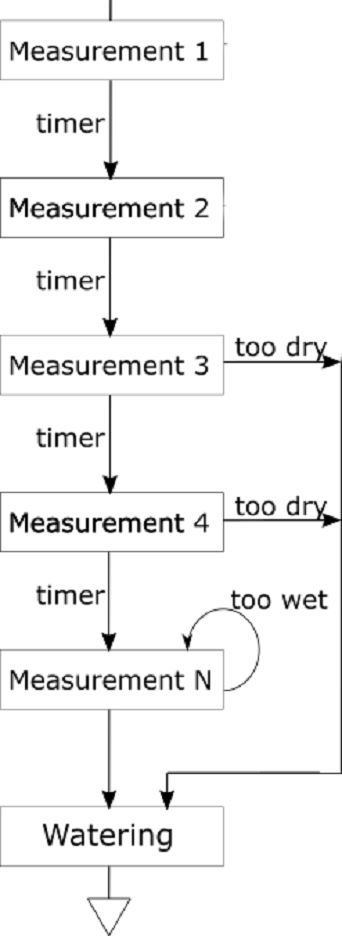
\includegraphics[width=0.3\textwidth]{marcel/algo}
    \label{arduinoalgo}
\end{wrapfigure}
In Abbildung \ref{arduinoalgo} ist der verwendete Bewässerungs-algorithmus zu sehen.
Nachdem das ESP-Programm einen Timerinterrupt an den Arduino gesendet hat,
startet dieser eine Messung an jeder Pflanze. Dabei wird auch ein Zähler
hochgesetzt. Sobald dieser einen einstellbaren Maximalwert erreicht wird
die Pflanze gegossen. Bei einen 8 Stunden Messintervall sind folgende
Bewässerungsrhythmen einstellbar: 1 Tag, 2 Tage, 7 Tage und 10 Tage.
Neben dem zeitbasierten System wird auch noch die Feuchtigkeit im Boden
der Pflanze einbezogen. Die letzten Messwerte der Pflanze werden gespeichert.
Wurde seit zwei Messungen nicht mehr gegossen, werden die letzten Messwerte
mit den voreingestellten Messwerten der Pflanze verglichen. Waren die
Messwerte unter der Trockengrenze wird eine verfrühte Bewässerung ausgeführt
und dabei der Zähler zurückgesetzt. Wird der maximale Zählerwert erreicht
werden die Messwerte mit dem Feuchtegrenzwert verglichen, sind sie zu hoch
und die Bewässerung ausgesetzt. Der Zähler wird dabei nicht zurückgesetzt,
sodass nach einen weiteren Timerinterrupt die Feuchte erneut getestet wird
und ggf. dann gegossen wird.

\newpage
\subsection{Programmablauf}
\begin{figure}
    \centering
    \includegraphics[width=0.9\textwidth]{marcel/ablauf}
    \caption{Ablauf des Programms}
\end{figure}
Nach dem Start des Arduinos wird zunächst das Setup durchlaufen, Alle Objekte mit
Startwerten initialisiert und das Hardwaresetup gemacht. Danach wird der Arduino
in den Sleep bzw. Energiesparmodus gebracht.  Sobald nun ein Interrupt des ESP an
den Arduino gesendet wird, erwacht dieser und erwartet einen Befehl am seriellen
Interface. Dieser wird ebenfalls vom ESP gesendet, um dann ausgewertet werden zu
können. Beinhaltet die Nachricht einen Befehl zum Ändern eines Wertes einer Pflanze,
wird dieser Wert geändert und der Arduino wieder in den Sparmodus versetzt. Handelt
es sich bei der Nachricht aber um einen Timerinterrupt, wird bei jeder Pflanze die
Routine gestartet. Wie bereits beschrieben, wird zunächst der zugehörige
Feuchtigkeitssensor ausgelesen, der Messungszähler erhöht und die vorliegende
Feuchtigkeit ausgewertet. Danach wird je nach Ergebnis der Auswertung der Sleep
Modus erneut gestartet oder mit der Bewässerung gestartet. Das Softwareobjekt
Pflanze schickt ein Signal an das zugehörige Ventil welches ein weiteres Signal
an die Pumpe schickt. Ist der Bewässerungsvorgang abgeschlossen, wird der Zähler
zurückgesetzt und der Energiesparmodus wird gestartet. 

\pagebreak
\fancyhf{}
\lhead{Michael Kainz}
\rhead{Seite \thepage}
\section{Software - ESP8266}
Der ESP8266 ist ein 32bit Mikrocontroller der Firma Espressif. Er besitzt ein integriertes
WIFI-Modul und in der verwendeten Version 1MB Flashspeicher.
\begin{figure}
    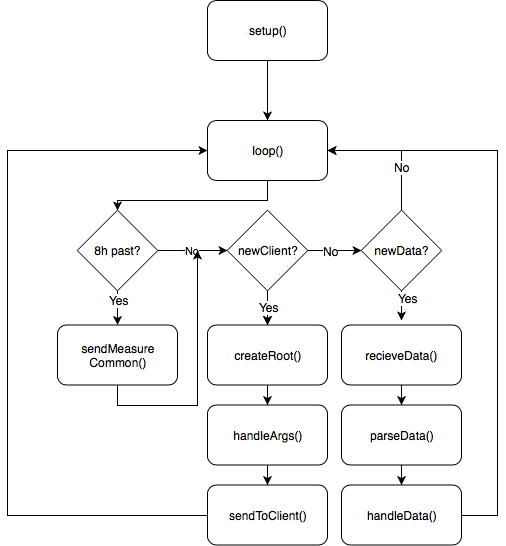
\includegraphics[width=\textwidth]{images/flow}
    \caption{Ablauf des ESP8266 Programms}
\end{figure}

\begin{tabular}{|l|l|}
    \hline
    Größen & Werte \\\hline
    Spannung & 2,5V..3,6V\\\hline
    Stromaufnahme & 2,5 $\mu$A..400mA\\\hline
    IO & 11..13 digitale Pins\\\hline
    Schnittstellen & SPI, UART, I$^2$C\\\hline
    Protokolle & TCP/IP v4 und v6, UDP, TCP\\\hline
    Datenrate & 150-300 kByte/s, Latenz ~10ms\\\hline

\end{tabular}

\subsection{Programmieren per Arduino IDE}
Der ESP8266 wird standardweise mit einem AT-Befehlssatz ausgeliefert, der für Modems und
Bluetooth-Module entwickelt wurde. Da der ESP8266 jedoch auch andere Aufgaben hat, als nur
dem Arduino als WIFI-Modul zu dienen, wurde eine neue Firmware geflasht und die Arduino IDE zum programmieren benutzt.
Das ermöglicht ein beschreiben des ESP8266 in C++, was es einfacher machte komplexe Abläufe
zu realisieren.
Dazu musste lediglich ein Zusatzpaket in der Arduino IDE heruntergeladen werden.

\subsection{Konfiguration}
Um den ESP8266 in Betrieb zu nehmen benötigt er die SSID und das Passwort des heimischen
Netzwerkes. Neben dem gewählten Client-Modus, kann der ESP8266 auch selbst als Server dienen.
Diese Funktion wurde nicht gewählt, da er zur Anzeige der Graphen und der Zeit eine
Internetverbindung braucht.

\section{Server}
Der Server zur Ansicht der Daten und Konfiguration der Anlage wird von dem ESP8266
Mikrocontroller bereitgestellt. Dieser verbindet sich mit dem heimischen Netzwerk.
Über die IP des ESP8266 kann man auf die Webseite zugreifen und bekommt die Graphen
zur Feuchtigkeit der Pflanzen sowie Einstellungsmöglichkeiten für beispielsweise Name
der Pflanze und gegossene Wassermenge angezeigt.

\subsection{Konfiguration}
Gestartet wird der Server durch $server.on(''/'', handleRoot);$ aus der Bibliothek \textit{ESP8266WebServer.h}. \textit{server} ist ein Objekt der ESP8266WebServer Klasse. Die Funktion teilt dem
Server mit, dass sobald sich ein Client auf den Root des Servers - also die IP-Adresse
des ESP8266 - verbindet, soll die Funktion \textit{handleRoot()} aufgerufen werden, die im Teil
Webseite (siehe \ref{handle}) erklärt wird.

Sollte ein User versuchen auf eine andere Seite als Root zugreifen wollen, wird die
Funktion \textit{handleNotFound()} aufgerufen. Dem User wird dann eine Error 404 Seite gezeigt,
die den versuchten Aufruf zeigt und dass dieser nicht gefunden werden konnte.

\subsection{Webseite}
Die Webseite für den User zeigt den Namen der jeweiligen Pflanzen an sowie Informationen
zur Feuchtigkeit und Einstellungsmöglichkeiten.
\begin{figure}[ht]
    \centering
    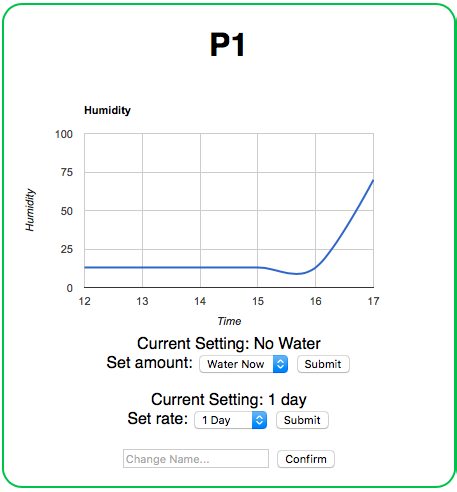
\includegraphics[width=0.7\textwidth]{images/seite2}
    \caption{Auszug der Webseite}
\end{figure}

\subsubsection{Graphen}
Die Graphen stellen den Wert der Feuchtigkeit aufgetragen über die Zeit dar. Die Daten
hierfür kommen direkt von den Sensoren des Arduino und werden vom ESP8266 in einem
Array gespeichert.
Das Array wird als DataTable an die Google Api weitergegeben. Von dort bekommt der User
den erstellten interaktiven Graphen übermittelt. Diese können durch Parameter wie Titel,
Kurventyp, Beschriftungen und Legenden verändert werden.
Dadurch, dass der Graph direkt an den User gesendet wird, entsteht auf dem ESP8266 keine
Last den Graphen zu erstellen oder zu speichern.

\subsubsection{Einstellbare Parameter}
Auf der Webseite befinden sich auch Parameter für jede Pflanze, die der User verändern kann.
Zur Personalisierung kann der angezeigte Name einer Pflanze geändert werden, beispielsweise
zur Art der zu überwachenden Pflanze. Dies geschieht über ein Textfeld, welches \textit{"Change Name..."}
anzeigt. Per Klick auf den \textit{"Confirm"} Button wird der neue Name übernommen und angezeigt.

Darüber hinaus kann die Häufigkeit und die Menge des Wassers, mit dem die trockene Pflanze gegossen werden soll,
auf vordefinierte Werte eingestellt werden.
Hierfür bietet ein Dropdown-Menü zusätzlich zu den Mengen
\textit{"Low"}, \textit{"Medium"} und \textit{"High"} auch \textit{"None"} und \textit{"Water now"} an. Somit ist es dem Benutzer möglich
bestimmte Pflanzen gar nicht oder auf Befehl bewässern zu lassen.

\subsubsection{Aufbau der Seite}
\label{handle}
Sobald der Benutzer die Webseite aufruft, arbeitet der ESP8266 die Funktion \textit{"handleRoot()"} ab.
Diese dient sowohl der Anpassung der internen Parameter als auch dem senden der Webseite an den Client.

Zuerst überprüft die Funktion ob die HTML-Anfrage einen POST-Teil aufweist und ob dieser
einen Parameter enthält. Sollte es ein Name sein, wird der alte Anzeigename durch den neuen
ersetzt. Ist der Parameter eine Wassermenge, wird außerdem das Argument des POSTs überprüft.
Darauf übermittelt der ESP8266 dem Arduino die neueingestellte Menge und passt seinerseits
den angezeigten Wert an.

Sobald die Überprüfungen der HTML-Anfrage abgeschlossen sind, wird die Funktion \textit{"createRoot()"}
aufgerufen. Diese erstellt aus den Parametern die fertige HTML-Seite, in dem Zeile für Zeile
ein String befüllt wird. Da der ESP8266 kein Filesystem von sich aus mitbringt, wurde diese
Methode benutzt um dem Benutzer eine interaktive Webseite präsentieren zu können.

Ist die Webseite erstellt, erfolgt eine Sendung des Strings an den Client.

\subsection{Network Time Protocol (NTP)}
Um eine regelmäßige Messung der Feuchtigkeit zu ermöglichen muss es eine Zeiteinheit geben,
die dem Arduino ein Signal gibt. Da weder der Arduino noch der ESP8266 eine Uhr eingebaut haben,
sondern nur die Zeit messen können, die seit dem letzten Boot verstrichen ist, wird ein NTP-Server
kontaktiert.
Dieser liefert jede Minute den exakten Epoch-Zeitwert. Dieser wird in das HH:mm DD.MM.YYYY Format
gebracht und mit den Messwerten des Arduino in die Arrays der Graphen gespeichert.

Zusätzlich wird an den Arduino nach einer gewissen Zeit ein Befehl zum Messen geschickt.
\section{Kommunikation}
Die Kommunikation zwischen dem ESP8266 und dem Arduino Uno erfolgt über UART (Universal Asynchronous Receiver Transmitter).
Über diese serielle Schnittstelle schickt der ESP8266 Befehle und konfigurierbare Parameter.
Der Arduino übermittelt Messwerte, die er von den Feuchtigkeitssensoren liest.
Um das zu ermöglichen wird jeweils der TX Port des einen Controllers mit dem RX Port des anderen verbunden.

\subsection{Funktionen}
Die verwendeten Nachrichten wurden in \ref{arduinokomm} aufgezeigt.
Folgende Funktionen ermöglichen die Kommunikation der beiden Mikrocontroller:
\newline



\begin{tabular}{|rl|p{5.5cm}|}
    \hline
    void & recvWithStartEndMarkers() & Filtert Eingang auf durch $<$ $>$ begrenzte Nachricht.\\\hline
    void & parseData() & Wertet Nachricht aus und extrahiert String und Integer.\\\hline
    void & serialHandler() & Verwaltet die extrahierten Daten.\\\hline
    String & clearFirstEntry(String) & Schiebt den ersten Wert im Array hinaus und füllt es mit dem Neuesten.\\\hline
    void & sendMessage(String, Int) & Gibt Arduino einen Interrupt, der auf Nachricht wartet.\\\hline
\end{tabular}


\newpage
\fancyhf{}
\rhead{Seite \thepage}
\section{Fazit}
Der Aufbau der Wasserversorgung war kniffliger als anfangs erwartet. Vor allem das
Auffinden der richtigen Fittings für die Gewinde mit den richtigen Durchmessern
stellte sich als Problem heraus. Nachdem die Probleme behoben waren,
funktionierte die geplante Versorgung aber einwandfrei und erfüllt die gestellten Anforderungen. 
Beim Aufbau der Energieversorgung ergaben sich nur Probleme beim Löten. So war der DC/DC-Wandler
mit seinen dünnen Stiften schwer einzulöten. Die geplante Schaltung verrichtet ihren Dienst, wie
erwartet. Im Nachhinein fallen noch
vergessene Details auf. So wäre ein Schalter für den Strom außen am Gehäuse von Vorteil gewesen.
Im Moment geht das System an, wenn das Netzteil eingesteckt wird. Auch das Verwenden von direkt
angelöteten Kabeln hat sich als nicht so
vorteilhaft herausgestellt. Steckerleisten wären wesentlich einfacher zu handhaben gewesen. Auch
die Ordnung im Elektrikkasten hätte sich dadurch erhöht.
Das Gehäuse ist für einen Prototypen vollkommen in Ordnung. Anpassbar wären noch passende Löcher
für Schalter und Steckerbuchsen.

Es  wäre  sinnvoller  gewesen,  die  Stromverteiler-  und
Leistungsschaltungsplatine  zu  kombinieren.  Dadurch  hätten  einige
Kabelverbindungen  weggelassen  werden  können  und  die  Übersicht
im  Elektronikkasten  verbessert  werden.  Um  den  Zusammenbau  und
die  Verkabelung  der  einzelnen  Platinen  zu  verbessern  wäre  es
hilfreich  gewesen,  nicht  alle  Kabel  fest  an  die  Platine  zu  löten,
sondern  alle  Verbindungen  mit  Hilfe  von  Stiftleisten  zu  realisieren.
So  hätten  beim  Zusammenbau  nur  die  Kabel  in  die  richtige  Stiftleiste
gesteckt  und  nicht  jedes  einzelne  Kabel  verlötet  werden  müssen.  Am
Ende  wurde  das  verlöten  der  Kabel  recht  umständlich,  da  das  Erreichen
der  Lötstelle  durch  die  vielen  bereits  vorhandenen  Kabel  erschwert  wird.
Zusätzlich  macht  dies  auch  eine  Reparatur  der  Platine  einfacher,  da  nur
alle  Kabel  abgezogen  und  nicht  abgelötet  werden  müssen.  Auch  hätte  die
die  Konstantanspannungsquelle  auf  den  Sensorplatinen  weggelassen  werden
können,  da  wir  die  Spannungsversorgung  mit  5V  extern  realisiert  haben.

Man sollte sich immer einen Überblick über die verfügbaren Pins des
Mikrocontrollers machen, da häufig bestimmte Funktionalitäten und an
bestimmten Pins verfügbar sind. Um im Nachhinein Pins innerhalb des Programms
noch zu ändern, sind Variable Adressen gegenüber festen Adressen sinnvoll.
Bei der Verwendung mehrerer Mikrocontroller ist stets auf ein einheitliches
Bezugspotential zu achten.

Zu Anfang wäre mehr Erfahrung mit dem ESP8266 sehr hilfreich gewesen.
Dadurch dass diese mit einer sehr kryptischen Firmware ausgeliefert werden,
gestalteten sich die ersten Schritte damit als sehr schwer. Doch sobald die alternative
Firmware geflasht wurde, konnte gut auf Fähigkeiten mit C/C++ zurückgegriffen werden.
Auch das Debuggen stellte sich als schwieriger als gedacht heraus. Es war kein Debugger
vorort den man hätte benutzen können, also wurde der Code via Serialausgaben verfolgt.
Dies ist ähnlich bei der Webseite an sich. Da diese in einem String gespeichert wurde und
dies die C-typischen Stolpersteinen war das Hinzufügen und Entfernen von Features herausfordernd.


\cleardoublepage
\phantomsection
\addcontentsline{toc}{section}{\listfigurename}

\listoffigures
\end{document}
%TODO: Autor in Fusszeile